\documentclass[landscape]{slides}
\usepackage{url}
\usepackage{amsmath}
\usepackage{graphicx}
\usepackage{color}
\usepackage{epic,ecltree}
\usepackage{qtree}
\usepackage{array}
%\usepackage{bar}
\usepackage{eclbip}
\usepackage{multicol}
\usepackage{algorithmic}
\usepackage{algorithm}
\renewcommand{\algorithmicrequire}{\textbf{Input:}}
\renewcommand{\algorithmicensure}{\textbf{Output:}}
\renewcommand{\algorithmiccomment}[1]{// {\em #1}}

\definecolor{darkblue}{rgb}{0,0,0.8}
\definecolor{darkgreen}{rgb}{0,0.8,0}
\definecolor{purple}{rgb}{0.6,0,0.6}
\definecolor{red}{rgb}{1,0,0}

\newcommand{\example}[1]{\textcolor{darkblue}{\rm #1}}
\newcommand{\maths}[1]{\textcolor{purple}{#1}}
\newcommand{\reference}[1]{\vspace{-2mm}\begin{flushright}\textcolor{purple}{\tiny [from #1]}\end{flushright}\vspace{-7mm}}
\newcommand{\bigref}[1]{\textcolor{purple}{[#1]}}

\begin{document}
\title[Chapter 11: Tree-Based Models]{Chapter 11\\[1cm] Tree-based models}
\author[Philipp Koehn]{}
\date{Statistical Machine Translation}

\maketitle

%%%%%%%%%%%%%%%%%%%%%%%%%%%%%%%%%%%%%%%%%%%%%%%%%%%%%%%%%%%%%%%%%%%%%%%%%%%%

\slide{Tree-Based Models}
\begin{itemize}\itemsep 10mm \vspace{10mm}
\item Traditional statistical models operate on sequences of words
\item Many translation problems can be best explained by pointing to syntax
\begin{itemize}
\item reordering, e.g., verb movement in German--English translation
\item long distance agreement (e.g., subject-verb) in output
\end{itemize}
\item[$\Rightarrow$] Translation models based on tree representation of language
\begin{itemize}
\item significant ongoing research
\item state-of-the art for some language pairs
\end{itemize}
\end{itemize}

%%%%%%%%%%%%%%%%%%%%%%%%%%%%%%%%%%%%%%%%%%%%%%%%%%%%%%%%%%%%%%%%%%%%%%%%%%%%

\slide{Phrase Structure Grammar}
\begin{itemize} \vspace{10mm}
\item Phrase structure
\begin{itemize}
\item noun phrases: \example{the big man}, \example{a house}, ...
\item prepositional phrases: \example{at 5 o'clock}, \example{in Edinburgh}, ...
\item verb phrases: \example{going out of business}, \example{eat chicken}, ...
\item adjective phrases, ...
\end{itemize}
\item Context-free Grammars (CFG)
\begin{itemize}
\item non-terminal symbols: phrase structure labels, part-of-speech tags
\item terminal symbols: words
\item production rules: \maths{\sc nt $\rightarrow$ [nt,t]+}\\
example: \example{\sc np $\rightarrow$ det nn}
\end{itemize}
\end{itemize}

%%%%%%%%%%%%%%%%%%%%%%%%%%%%%%%%%%%%%%%%%%%%%%%%%%%%%%%%%%%%%%%%%%%%%%%%%%%%

\slide{Phrase Structure Grammar}
\begin{center}
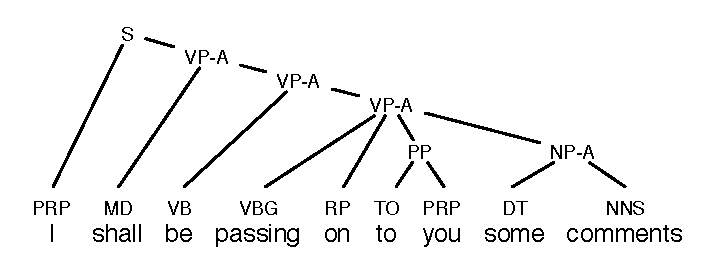
\includegraphics[width=25cm]{tree-psg.pdf}\\[5mm]
Phrase structure grammar tree for an English sentence\\ 
(as produced Collins' parser)
\end{center}

%%%%%%%%%%%%%%%%%%%%%%%%%%%%%%%%%%%%%%%%%%%%%%%%%%%%%%%%%%%%%%%%%%%%%%%%%%%%

\slide{Synchronous Phrase Structure Grammar}
\begin{itemize} \vspace{10mm}
\item English rule
\begin{center}
\example{\sc np $\rightarrow$ det jj nn}
\end{center}
\item French rule
\begin{center}
\example{\sc np $\rightarrow$ det nn jj}
\end{center}
\item Synchronous rule (indices indicate alignment):
\begin{center}
\example{{\sc np} $\rightarrow$ $\text{\sc det}_1$ $\text{\sc nn}_2$ $\text{\sc jj}_3\;|\;\text{\sc det}_1$ $\text{\sc jj}_3$ $\text{\sc nn}_2$}
\end{center}
\end{itemize}

%%%%%%%%%%%%%%%%%%%%%%%%%%%%%%%%%%%%%%%%%%%%%%%%%%%%%%%%%%%%%%%%%%%%%%%%%%%%

\slide{Synchronous Grammar Rules}
\begin{itemize}\vspace{10mm}
\item Nonterminal rules\vspace{-5mm}
\begin{center}
\example{{\sc np} $\rightarrow$ $\text{\sc det}_1$ $\text{\sc nn}_2$ $\text{\sc jj}_3\;|\;\text{\sc det}_1$ $\text{\sc jj}_3$ $\text{\sc nn}_2$}
\end{center}
\item Terminal rules\vspace{-5mm}
\example{\begin{center}
{\sc n} $\rightarrow$ maison $\;|\;$ house\\[4mm]
{\sc np} $\rightarrow$ la maison bleue $\;|\;$ the blue house
\end{center}}
\item Mixed rules\vspace{-5mm}
\begin{center}
\example{{\sc np} $\rightarrow$ la maison $\text{\sc jj}_1\;|\;$ the $\text{\sc jj}_1$ house}
\end{center}
\end{itemize}

%%%%%%%%%%%%%%%%%%%%%%%%%%%%%%%%%%%%%%%%%%%%%%%%%%%%%%%%%%%%%%%%%%%%%%%%%%%%

\slide{Tree-Based Translation Model}
\begin{itemize}\vspace{10mm}
\item Translation by parsing
\begin{itemize}
\item synchronous grammar has to parse entire input sentence
\item output tree is generated at the same time
\item process is broken up into a number of rule applications
\end{itemize}
\item Translation probability
\maths{\begin{equation*}
\text{\sc score}(\text{\sc tree}, \text{\sc e}, \text{\sc f}) = \prod_i \text{\sc rule}_i
\end{equation*}}\vspace{-17mm}
\item Many ways to assign probabilities to rules
\end{itemize}

%%%%%%%%%%%%%%%%%%%%%%%%%%%%%%%%%%%%%%%%%%%%%%%%%%%%%%%%%%%%%%%%%%%%%%%%%%%%

\slide{Aligned Tree Pair}
\begin{center}
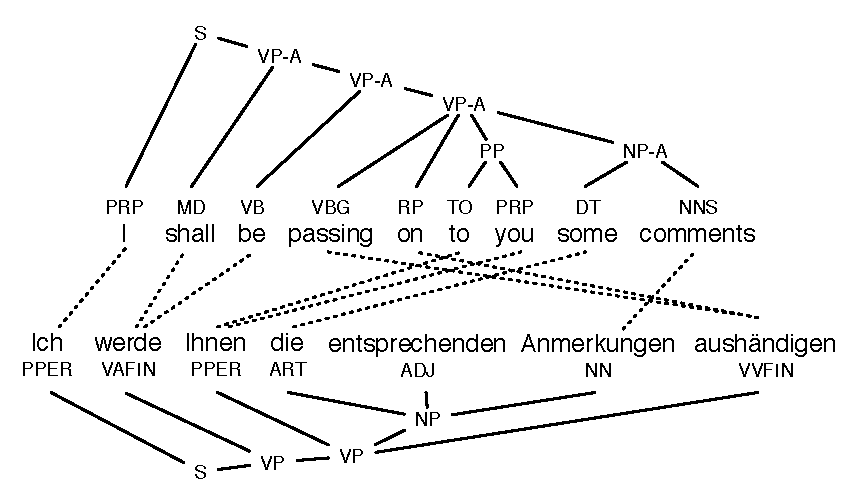
\includegraphics[width=19cm]{tree-aligned.pdf}\\[5mm]
Phrase structure grammar trees with word alignment\\
(German--English sentence pair.)
\end{center}

%%%%%%%%%%%%%%%%%%%%%%%%%%%%%%%%%%%%%%%%%%%%%%%%%%%%%%%%%%%%%%%%%%%%%%%%%%%%

\slide{Reordering Rule}
\begin{itemize}
\item Subtree alignment\vspace{-8mm}
\example{\begin{center} 
\Tree [.{\sc vp} \qroof{...}.{\sc pper} \qroof{...}.{\sc np} [.{\sc vvfin} aush{\"a}ndigen ] ]
\hspace{5mm} {\Large $\leftrightarrow$} \hspace{5mm}
\Tree [.{\sc vp} [.{\sc vbg} passing ] [.{\sc rp} on ] \qroof{...}.{\sc pp} \qroof{...}.{\sc np} ] 
\end{center}} \vspace{-5mm}
\item Synchronous grammar rule\vspace{-8mm}
\begin{center} 
\example{{\sc vp} $\rightarrow$ $\text{\sc pper}_1$ $\text{\sc np}_2$ aush{\"a}ndigen $\;|\;$ passing on $\text{\sc pp}_1$ $\text{\sc np}_2$}
\end{center}
\item Note: 
\begin{itemize}
\item one word \example{aush{\"a}ndigen} mapped to two words \example{passing on} ok
\item but: fully non-terminal rule not possible\\ (one-to-one mapping constraint for nonterminals)
\end{itemize}
\end{itemize}

%%%%%%%%%%%%%%%%%%%%%%%%%%%%%%%%%%%%%%%%%%%%%%%%%%%%%%%%%%%%%%%%%%%%%%%%%%%%

\slide{Another Rule}
\begin{itemize}
\item Subtree alignment\vspace{-5mm}
\example{\begin{center}
\Tree [.{\sc pro} Ihnen ] 
\hspace{15mm} {\Large $\leftrightarrow$} \hspace{15mm}
\Tree [.{\sc pp} [.{\sc to} to ] [.{\sc prp} you ] ] 
\end{center}} \vspace{-5mm}
\item Synchronous grammar rule (stripping out English internal structure)
\example{\begin{center}
{\sc pro/pp} $\rightarrow$ Ihnen $\;|\;$ to you
\end{center}}
\item Rule with internal structure
\example{\begin{center}
\newcolumntype{S}[1]{>{\centering\arraybackslash} m{#1} }
\begin{tabular}{S{19mm}S{2mm}S{26mm}|S{36mm}} 
{\sc pro/pp} & $\rightarrow$ &
Ihnen & 
\Tree [.{\sc to} to ] $\;\;$ \Tree [.{\sc prp} you ]
\vspace{-4.5mm}\phantom{.}
\end{tabular}
\end{center}}
\end{itemize}

%%%%%%%%%%%%%%%%%%%%%%%%%%%%%%%%%%%%%%%%%%%%%%%%%%%%%%%%%%%%%%%%%%%%%%%%%%%%

\slide{Another Rule}
\begin{itemize}
\item Translation of German \example{werde} to English \example{shall be}
\example{\begin{center}
\Tree [.{\sc vp} [.{\sc vafin} werde ] \qroof{...}.{\sc vp} ]
\hspace{15mm} {\Large $\leftrightarrow$} \hspace{15mm}
\Tree [.{\sc vp} [.{\sc md} shall ] [.{\sc vp} [.{\sc vb} be ] \qroof{...}.{\sc vp} ] ] 
\end{center}} \vspace{-11mm}
\item Translation rule needs to include mapping of \example{\sc vp}
\item[$\Rightarrow$] Complex rule\vspace{-10mm}
\example{\begin{center}
\newcolumntype{S}[1]{>{\centering\arraybackslash} m{#1} }
\begin{tabular}{S{7mm}S{7mm}S{40mm}|S{68mm}} %\usepackage{array}
{\sc vp} & $\rightarrow$ &
\Tree [.{\sc vafin} werde ] $\;\;$ $\text{\sc vp}_1$
\vspace{-2mm}\phantom{.} &
\Tree [.{\sc md} shall ] $\;\;$ \Tree [.{\sc vp} [.{\sc vb} be ] $\text{\sc vp}_1$ ]
\vspace{-9mm}\phantom{.}
\end{tabular}
\end{center}}
\end{itemize}

%%%%%%%%%%%%%%%%%%%%%%%%%%%%%%%%%%%%%%%%%%%%%%%%%%%%%%%%%%%%%%%%%%%%%%%%%%%%

\slide{Internal Structure}
\begin{itemize}
\item Stripping out internal structure
\begin{center}
\example{{\sc vp} $\rightarrow$ werde $\text{\sc vp}_1$ $\;|\;$ shall be $\text{\sc vp}_1$ }
\end{center}
$\Rightarrow$ synchronous context free grammar\vspace{5mm}
\item Maintaining internal structure
\example{\begin{center}
\newcolumntype{S}[1]{>{\centering\arraybackslash} m{#1} }
\begin{tabular}{S{7mm}S{7mm}S{40mm}|S{68mm}} %\usepackage{array}
{\sc vp} & $\rightarrow$ &
\Tree [.{\sc vafin} werde ] $\;\;$ $\text{\sc vp}_1$
\vspace{-2mm}\phantom{.} &
\Tree [.{\sc md} shall ] $\;\;$ \Tree [.{\sc vp} [.{\sc vb} be ] $\text{\sc vp}_1$ ]
\vspace{-9mm}\phantom{.}
\end{tabular}
\end{center}}
$\Rightarrow$ synchronous tree substitution grammar
\end{itemize}

%%%%%%%%%%%%%%%%%%%%%%%%%%%%%%%%%%%%%%%%%%%%%%%%%%%%%%%%%%%%%%%%%%%%%%%%%%%%

\slide{Learning Synchronous Grammars}
\begin{itemize}\vspace{10mm}\itemsep 10mm
\item Extracting rules from a word-aligned parallel corpus
\item First: Hierarchical phrase-based model
\begin{itemize}
\item only one non-terminal symbol \example{\sc x}
\item no linguistic syntax, just a formally syntactic model
\end{itemize}
\item Then: Synchronous phrase structure model
\begin{itemize}
\item non-terminals for words and phrases: \example{\sc np, vp, pp, adj, ...}
\item corpus must also be parsed with syntactic parser
\end{itemize}
\end{itemize}

%%%%%%%%%%%%%%%%%%%%%%%%%%%%%%%%%%%%%%%%%%%%%%%%%%%%%%%%%%%%%%%%%%%%%%%%%%%%

\slide{Extracting Phrase Translation Rules}
\begin{center}
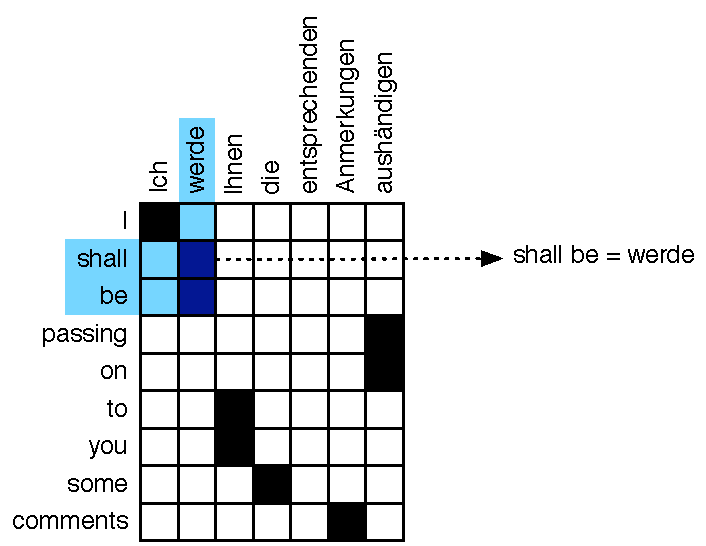
\includegraphics[scale=1.4]{hierarchical-phrase-extraction1.pdf}
\end{center}

%%%%%%%%%%%%%%%%%%%%%%%%%%%%%%%%%%%%%%%%%%%%%%%%%%%%%%%%%%%%%%%%%%%%%%%%%%%%

\slide{Extracting Phrase Translation Rules}
\begin{center}
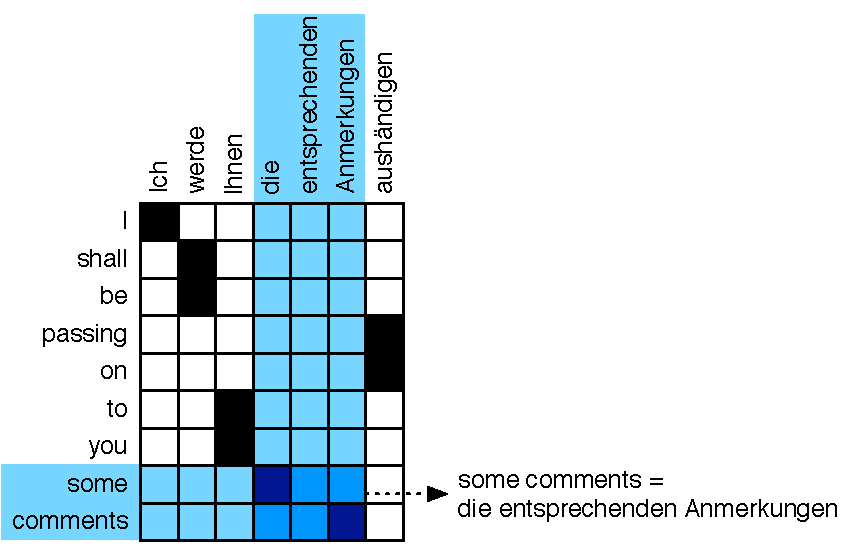
\includegraphics[scale=1.4]{hierarchical-phrase-extraction2.pdf}
\end{center}

%%%%%%%%%%%%%%%%%%%%%%%%%%%%%%%%%%%%%%%%%%%%%%%%%%%%%%%%%%%%%%%%%%%%%%%%%%%%

\slide{Extracting Phrase Translation Rules}
\begin{center}
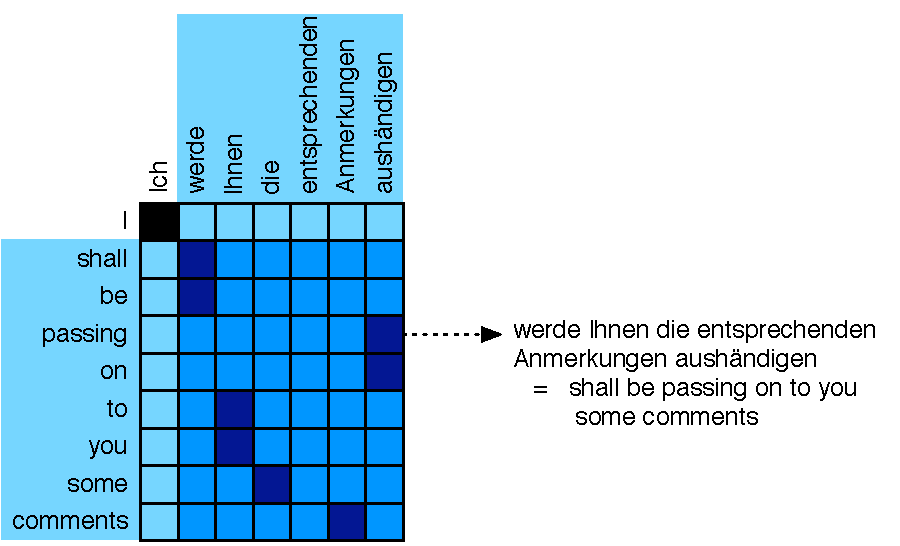
\includegraphics[scale=1.4]{hierarchical-phrase-extraction3.pdf}
\end{center}

%%%%%%%%%%%%%%%%%%%%%%%%%%%%%%%%%%%%%%%%%%%%%%%%%%%%%%%%%%%%%%%%%%%%%%%%%%%%

\slide{Extracting Hierarchical Phrase Translation Rules}
\begin{center}
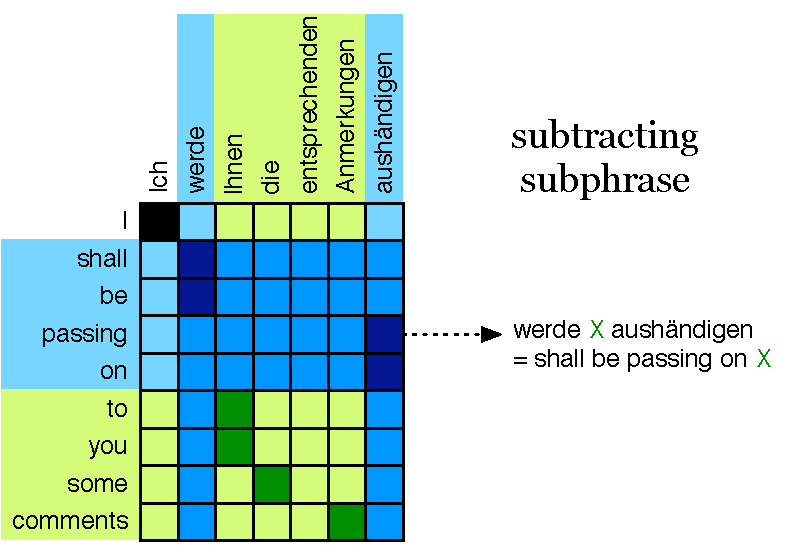
\includegraphics[scale=1.4]{hierarchical-phrase-extraction4.pdf}
\end{center}

%%%%%%%%%%%%%%%%%%%%%%%%%%%%%%%%%%%%%%%%%%%%%%%%%%%%%%%%%%%%%%%%%%%%%%%%%%%%

\slide{Formal Definition}
\begin{itemize}\vspace{15mm}
\item Recall: consistent phrase pairs
\maths{\begin{equation*}
\begin{split}
( \bar{e} , \bar{f} ) \; \mbox{consistent with} & \; A \Leftrightarrow \\
 & \forall e_i \in \bar{e}: (e_i,f_j) \in A \rightarrow f_j \in \bar{f} \\
 \mbox{\sc and} & \; \forall f_j \in \bar{f}: (e_i,f_j) \in A \rightarrow e_i  \in \bar{e} \\
 \mbox{\sc and} & \; \exists e_i \in \bar{e}, f_j \in \bar{f}: (e_i,f_j) \in A
\end{split}
\end{equation*}}
\item Let \maths{$P$} be the set of all extracted phrase pairs \maths{$( \bar{e} , \bar{f} )$}
\end{itemize}

%%%%%%%%%%%%%%%%%%%%%%%%%%%%%%%%%%%%%%%%%%%%%%%%%%%%%%%%%%%%%%%%%%%%%%%%%%%%

\slide{Formal Definition}
\begin{itemize}\vspace{10mm}
\item Extend recursively:
\maths{\begin{equation*}
\begin{split}
\text{if}\; & ( \bar{e} , \bar{f} ) \in P \;\mbox{\sc and}\; ( \bar{e}_\text{\sc sub} , \bar{f}_\text{\sc sub} ) \in P \\
& \phantom{.} \hspace{1cm} \mbox{\sc and}\; \bar{e} = \bar{e}_\text{\sc pre}+\bar{e}_\text{\sc sub}+\bar{e}_\text{\sc post} \\
& \phantom{.} \hspace{1cm} \mbox{\sc and}\; \bar{f} = \bar{f}_\text{\sc pre}+\bar{f}_\text{\sc sub}+\bar{f}_\text{\sc post} \\
& \phantom{.} \hspace{1cm} \mbox{\sc and}\; \bar{e} \ne \bar{e}_\text{\sc sub} \;\text{\sc and}\; \bar{f} \ne \bar{f}_\text{\sc sub} \\
\text{add}\; & (e_\text{\sc pre}+\text{\sc x}+e_\text{\sc post},f_\text{\sc pre}+\text{\sc x}+f_\text{\sc post}) \;\text{to}\; P
\end{split}
\end{equation*}}
(note: any of \maths{$e_\text{\sc pre}$}, \maths{$e_\text{\sc post}$}, \maths{$f_\text{\sc pre}$}, or \maths{$f_\text{\sc post}$} may be empty)
\item Set of hierarchical phrase pairs is the closure under this extension mechanism
\end{itemize}

%%%%%%%%%%%%%%%%%%%%%%%%%%%%%%%%%%%%%%%%%%%%%%%%%%%%%%%%%%%%%%%%%%%%%%%%%%%%

\slide{Comments}
\begin{itemize}\vspace{15mm}
\item Removal of multiple sub-phrases leads to rules with multiple non-terminals, such as:
\begin{center}
\example{{\sc y} $\rightarrow$ $\text{\sc x}_1$ $\text{\sc x}_2$ $\;|\;$ $\text{\sc x}_2$ {\em of} $\text{\sc x}_1$}
\end{center}
\item Typical restrictions to limit complexity \bigref{Chiang, 2005}
\begin{itemize} \itemsep -3pt
\item at most 2 nonterminal symbols
\item at least 1 but at most 5 words per language 
\item span at most 15 words (counting gaps)
\end{itemize}

\end{itemize}

%%%%%%%%%%%%%%%%%%%%%%%%%%%%%%%%%%%%%%%%%%%%%%%%%%%%%%%%%%%%%%%%%%%%%%%%%%%%

\slide{Learning Syntactic Translation Rules}
\begin{center}
\begin{tabular}{rl}
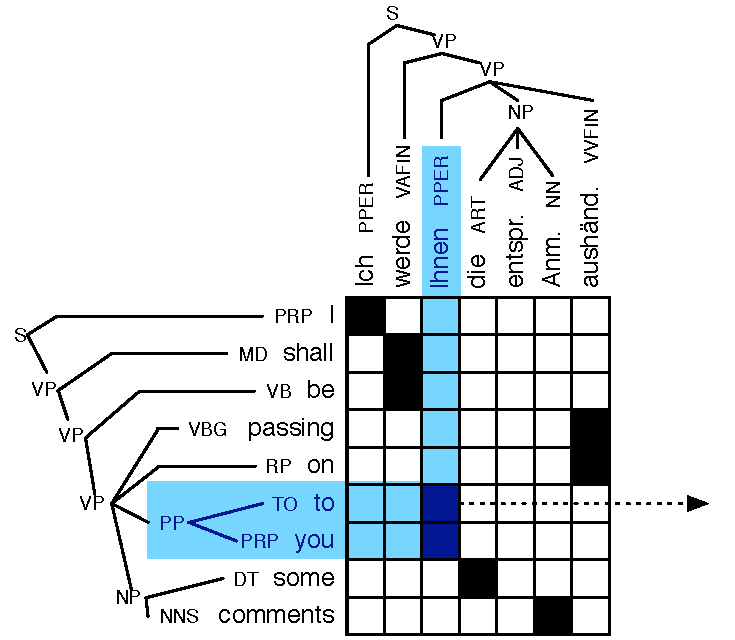
\includegraphics[scale=1.17]{hierarchical-phrase-extraction-syntax1.pdf}
& 
\parbox{85mm}{\footnotesize \phantom{.}\vspace{-6cm}

\example{\Tree [.{\sc pro} Ihnen ] }
\hspace{2mm} {\Large $=$} \hspace{2mm}
\example{\Tree [.{\sc pp} [.{\sc to} to ] [.{\sc prp} you ] ] \vspace{-1cm}\phantom{.}}
}
\end{tabular}
\end{center}

%%%%%%%%%%%%%%%%%%%%%%%%%%%%%%%%%%%%%%%%%%%%%%%%%%%%%%%%%%%%%%%%%%%%%%%%%%%%

\slide{Constraints on Syntactic Rules}
\vspace{15mm}
\begin{itemize}
\item Same word alignment constraints as hierarchical models
\item Hierarchical: rule can cover any span\\
$\Leftrightarrow$ syntactic rules must cover constituents in the tree
\item Hierarchical: gaps may cover any span\\
$\Leftrightarrow$ gaps must cover constituents in the tree
\vspace{10mm}
\item Much less rules are extracted (all things being equal)
\end{itemize}

%%%%%%%%%%%%%%%%%%%%%%%%%%%%%%%%%%%%%%%%%%%%%%%%%%%%%%%%%%%%%%%%%%%%%%%%%%%%

\slide{Impossible Rules}
\begin{center}
\begin{tabular}{rl}
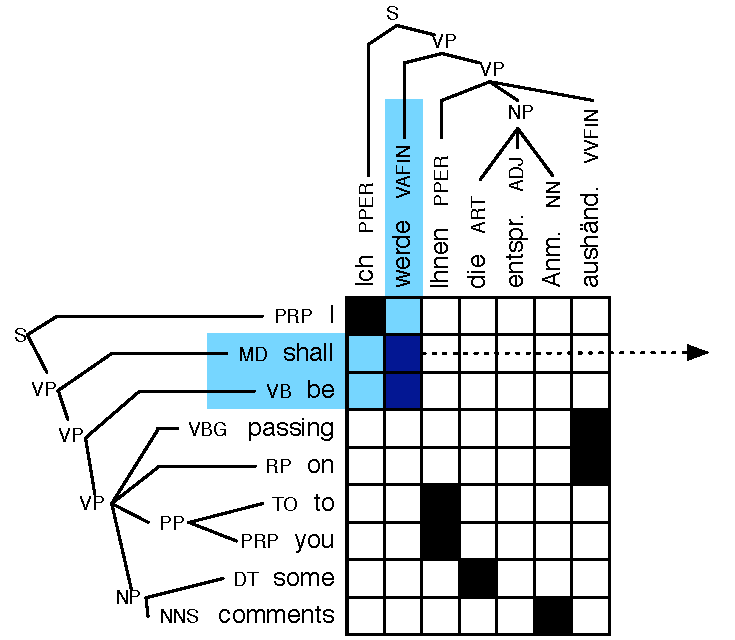
\includegraphics[scale=1.17]{hierarchical-phrase-extraction-syntax2.pdf}
& 
\parbox{95mm}{ \phantom{.}\vspace{-11cm}
English span not a constituent\\
no rule extracted
}
\end{tabular}
\end{center}


%%%%%%%%%%%%%%%%%%%%%%%%%%%%%%%%%%%%%%%%%%%%%%%%%%%%%%%%%%%%%%%%%%%%%%%%%%%%

\slide{Rules with Context}
\begin{center}
\begin{tabular}{rl}
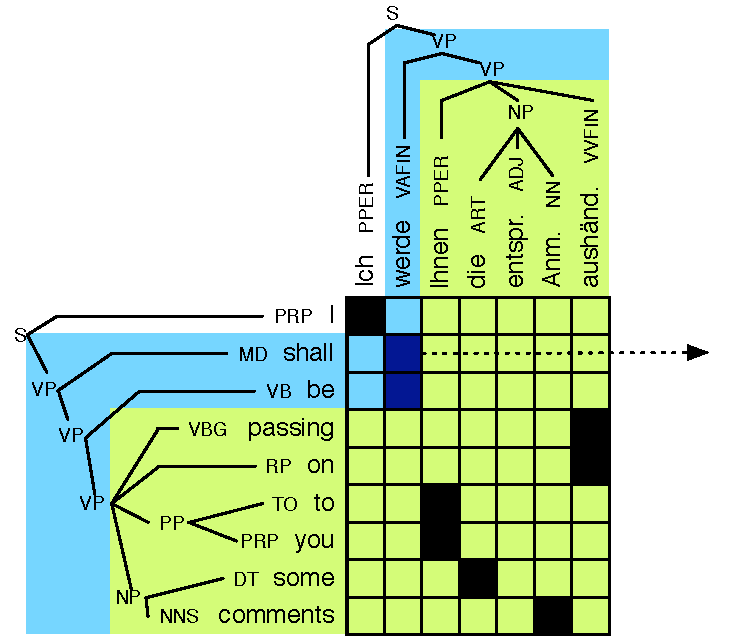
\includegraphics[scale=1.17]{hierarchical-phrase-extraction-syntax3.pdf}
& 
\parbox{95mm}{\phantom{.}\vspace{-11cm}
Rule with this phrase pair\\[3mm]
requires syntactic context\\[-1cm]
\footnotesize 
\example{\Tree [.{\sc vp} [.{\sc vafin} werde ] \qroof{...}.{\sc vp} ]}
\hspace{2mm} \parbox{5mm}{\phantom{.} 

\vspace{39mm}{\Large $=$}} \hspace{2mm}
\example{\Tree [.{\sc vp} [.{\sc md} shall ] [.{\sc vp} [.{\sc vb} be ] \qroof{...}.{\sc vp} ] ] }
}
\end{tabular}
\end{center}

%%%%%%%%%%%%%%%%%%%%%%%%%%%%%%%%%%%%%%%%%%%%%%%%%%%%%%%%%%%%%%%%%%%%%%%%%%%%

\slide{Too Many Rules Extractable}
\vspace{20mm}
\begin{itemize}\itemsep 5mm
\item Huge number of rules can be extracted\\
{\small (every alignable node may or may not be part of a rule $\rightarrow$ exponential number of rules)}
\item Need to limit which rules to extract
\vspace{5mm}
\item Option 1: similar restriction as for hierarchical model\\
{\small (maximum span size, maximum number of terminals and non-terminals, etc.)}
\item Option 2: only extract minimal rules ("GHKM" rules)
\end{itemize}

%%%%%%%%%%%%%%%%%%%%%%%%%%%%%%%%%%%%%%%%%%%%%%%%%%%%%%%%%%%%%%%%%%%%%%%%%%%%

\slide{Minimal Rules}
\vspace{5mm}
\begin{center}
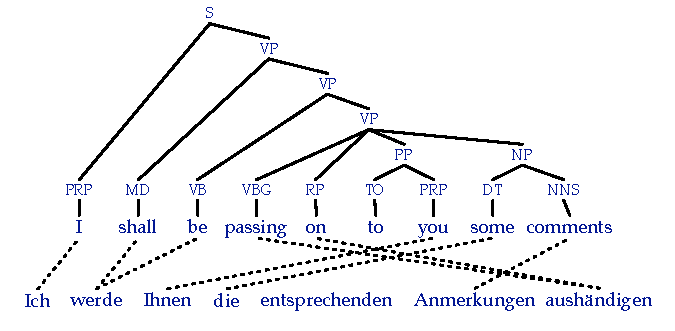
\includegraphics[scale=2.1]{minimal-rules0.pdf}\\[5mm]
Extract: set of smallest rules required to explain the sentence pair
\end{center}

%%%%%%%%%%%%%%%%%%%%%%%%%%%%%%%%%%%%%%%%%%%%%%%%%%%%%%%%%%%%%%%%%%%%%%%%%%%%

\slide{Lexical Rule}
\vspace{5mm}
\begin{center}
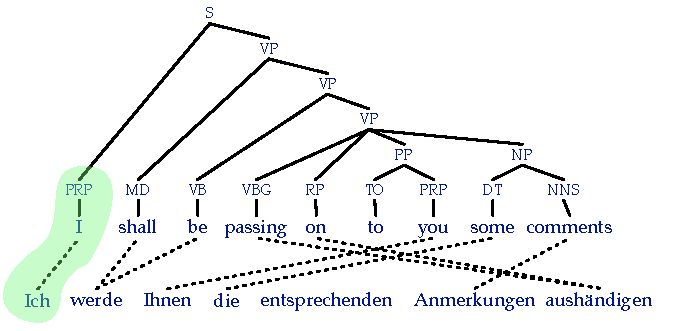
\includegraphics[scale=2.1]{minimal-rules1.pdf}\\[5mm]
Extracted rule: \example{{\sc prp} $\rightarrow$ Ich $|$ I}
\end{center}

%%%%%%%%%%%%%%%%%%%%%%%%%%%%%%%%%%%%%%%%%%%%%%%%%%%%%%%%%%%%%%%%%%%%%%%%%%%%

\slide{Lexical Rule}
\vspace{5mm}
\begin{center}
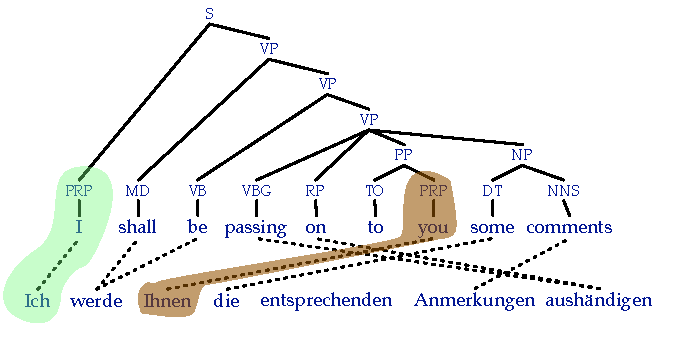
\includegraphics[scale=2.1]{minimal-rules2.pdf}\\
Extracted rule: \example{{\sc prp} $\rightarrow$ Ihnen $|$ you}
\end{center}

%%%%%%%%%%%%%%%%%%%%%%%%%%%%%%%%%%%%%%%%%%%%%%%%%%%%%%%%%%%%%%%%%%%%%%%%%%%%

\slide{Lexical Rule}
\vspace{5mm}
\begin{center}
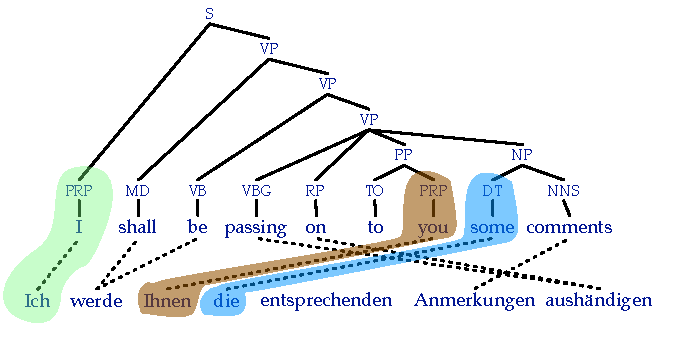
\includegraphics[scale=2.1]{minimal-rules3.pdf}\\[-1mm]
Extracted rule: \example{{\sc dt} $\rightarrow$ die $|$ some}
\end{center}

%%%%%%%%%%%%%%%%%%%%%%%%%%%%%%%%%%%%%%%%%%%%%%%%%%%%%%%%%%%%%%%%%%%%%%%%%%%%

\slide{Lexical Rule}
\vspace{5mm}
\begin{center}
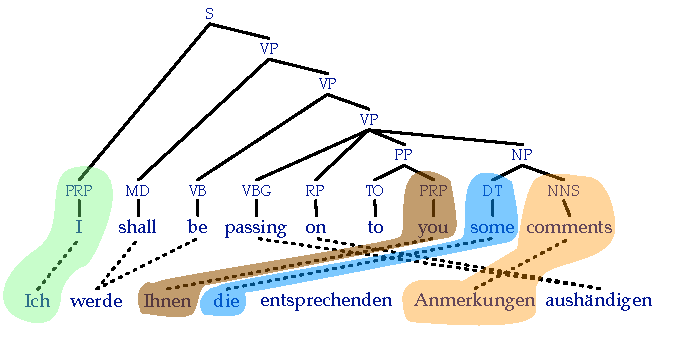
\includegraphics[scale=2.1]{minimal-rules4.pdf}\\[-1mm]
Extracted rule: \example{{\sc nns} $\rightarrow$ Anmerkungen $|$ comments}
\end{center}

%%%%%%%%%%%%%%%%%%%%%%%%%%%%%%%%%%%%%%%%%%%%%%%%%%%%%%%%%%%%%%%%%%%%%%%%%%%%

\slide{Insertion Rule}
\vspace{5mm}
\begin{center}
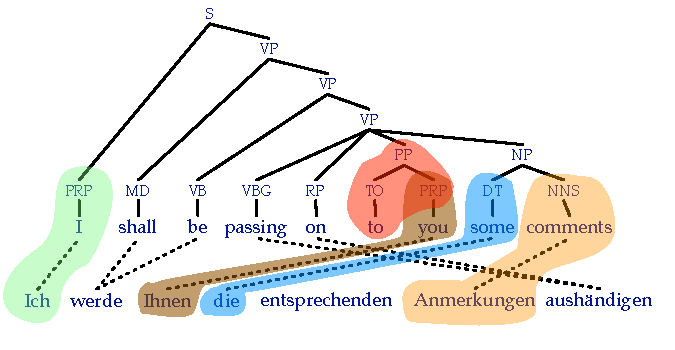
\includegraphics[scale=2.1]{minimal-rules5.pdf}\\[-1mm]
Extracted rule: \example{{\sc pp} $\rightarrow$ {\sc x} $|$ to {\sc prp}}
\end{center}

%%%%%%%%%%%%%%%%%%%%%%%%%%%%%%%%%%%%%%%%%%%%%%%%%%%%%%%%%%%%%%%%%%%%%%%%%%%%

\slide{Non-Lexical Rule}
\vspace{5mm}
\begin{center}
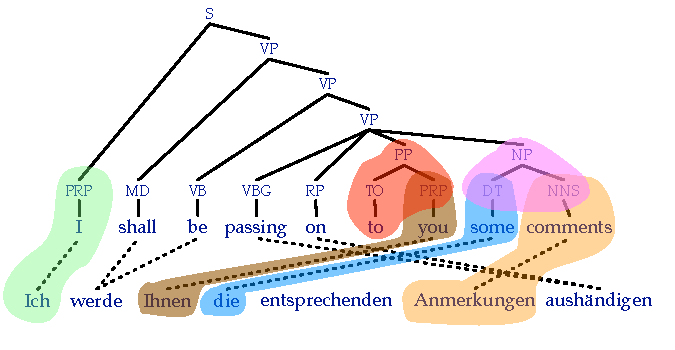
\includegraphics[scale=2.1]{minimal-rules6.pdf}\\[-1mm]
Extracted rule: \example{{\sc np} $\rightarrow$ $\text{\sc x}_1$ $\text{\sc x}_2$ $|$ $\text{\sc dt}_1$ $\text{\sc nns}_2$}
\end{center}

%%%%%%%%%%%%%%%%%%%%%%%%%%%%%%%%%%%%%%%%%%%%%%%%%%%%%%%%%%%%%%%%%%%%%%%%%%%%

\slide{Lexical Rule with Syntactic Context}
\vspace{3mm}
\begin{center}
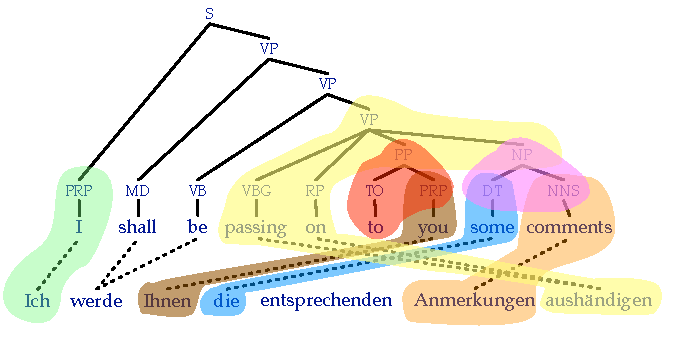
\includegraphics[scale=2.1]{minimal-rules7.pdf}\\[-1mm]
Extracted rule: \example{{\sc vp} $\rightarrow$ $\text{\sc x}_1$ $\text{\sc x}_2$ aush{\"a}ndigen $|$ passing on $\text{\sc pp}_1$ $\text{\sc np}_2$}
\end{center}

%%%%%%%%%%%%%%%%%%%%%%%%%%%%%%%%%%%%%%%%%%%%%%%%%%%%%%%%%%%%%%%%%%%%%%%%%%%%

\slide{Lexical Rule with Syntactic Context}
\vspace{3mm}
\begin{center}
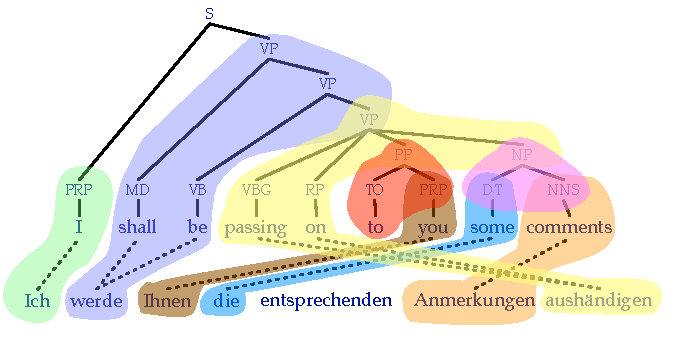
\includegraphics[scale=2.1]{minimal-rules8.pdf}\\[-1mm]
Extracted rule: \example{{\sc vp} $\rightarrow$ werde  {\sc x} $|$ shall be {\sc vp}} (ignoring internal structure)
\end{center}

%%%%%%%%%%%%%%%%%%%%%%%%%%%%%%%%%%%%%%%%%%%%%%%%%%%%%%%%%%%%%%%%%%%%%%%%%%%%

\slide{Non-Lexical Rule}
\vspace{-4mm}
\begin{center}
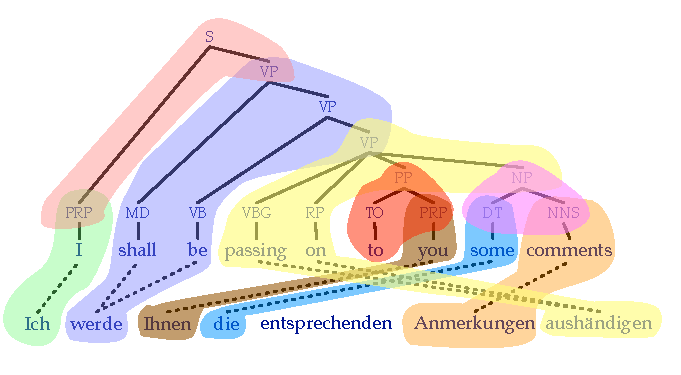
\includegraphics[scale=2.1]{minimal-rules9.pdf}\\[-9mm]
Extracted rule: \example{{\sc s} $\rightarrow$ $\text{\sc x}_1$ $\text{\sc x}_2$ $|$ $\text{\sc prp}_1$ $\text{\sc vp}_2$}\\
{\sc done} --- note: one rule per alignable constituent
\end{center}

%%%%%%%%%%%%%%%%%%%%%%%%%%%%%%%%%%%%%%%%%%%%%%%%%%%%%%%%%%%%%%%%%%%%%%%%%%%%

\slide{Unaligned Source Words}
\vspace{-6mm}
\begin{center}
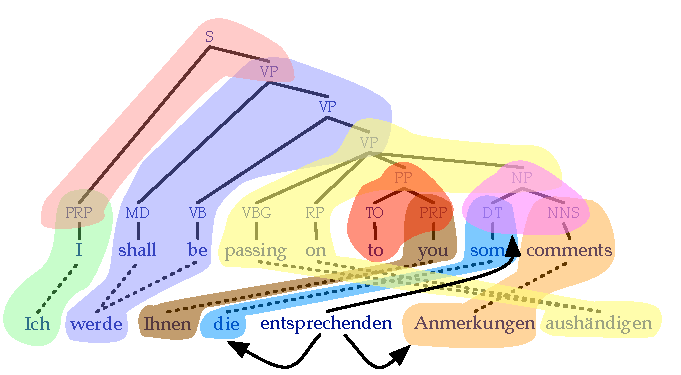
\includegraphics[scale=2.1]{minimal-rules-unaligned.pdf}\\[-1mm]
Attach to neighboring words or higher nodes $\rightarrow$ additional rules
\end{center}

%%%%%%%%%%%%%%%%%%%%%%%%%%%%%%%%%%%%%%%%%%%%%%%%%%%%%%%%%%%%%%%%%%%%%%%%%%%%

\slide{Too Few Phrasal Rules?}
\vspace{20mm}
\begin{itemize}\itemsep 10mm
\item Lexical rules will be 1-to-1 mappings (unless word alignment requires otherwise)
\item But: phrasal rules very beneficial in phrase-based models
\item Solutions
\begin{itemize}
\item combine rules that contain a maximum number of symbols\\
(as in hierarchical models, recall: "Option 1")
\vspace{5mm}
\item compose minimal rules to cover a maximum number of non-leaf nodes
\end{itemize}
\end{itemize}

%%%%%%%%%%%%%%%%%%%%%%%%%%%%%%%%%%%%%%%%%%%%%%%%%%%%%%%%%%%%%%%%%%%%%%%%%%%%

\slide{Composed Rules}
\begin{itemize}
\item Current rules\vspace{-2cm}
\begin{center}
\example{$\text{\sc x}_1$ $\text{\sc x}_2$
\hspace{2mm} = \hspace{-95mm}
\Tree [.{\sc np} $\text{\sc dt}_1$ $\text{\sc nns}_1$ ] }\\[1cm]
%
\example{die
\hspace{2mm} = \hspace{-15mm}
\Tree [.{\sc dt} some ]}
%
\hspace{3cm}
\example{entsprechenden Anmerkungen
\hspace{2mm} = \hspace{-25mm}
\Tree [.{\sc nns} comments ]}\\
\end{center}

\item Composed rule
\vspace{-1cm}
\begin{center}
\example{die entsprechenden Anmerkungen
\hspace{2mm} = \hspace{-55mm}
\Tree [.{\sc \textcolor{red}{np}} [.{\sc dt} some ]  [.{\sc nns} comments ] ] }\\[3mm]
(1 non-leaf node: \example{\textcolor{red}{\sc np}})
\end{center}
\end{itemize}

%%%%%%%%%%%%%%%%%%%%%%%%%%%%%%%%%%%%%%%%%%%%%%%%%%%%%%%%%%%%%%%%%%%%%%%%%%%%

\slide{Composed Rules}
\begin{itemize}
\item Minimal rule: \hspace{2cm}
\example{$\text{\sc x}_1$ $\text{\sc x}_2$ aush{\"a}ndigen
\hspace{2mm} = \hspace{-55mm}
\Tree [.{\sc \textcolor{red}{vp}} [.{\sc prp} passing ]  [.{\sc prp} on ]  $\text{\sc \textcolor{red}{pp}}_1$ $\text{\sc \textcolor{red}{np}}_2$ ] }\\[-15mm]
 3 non-leaf nodes:\\ \example{\textcolor{red}{\sc vp}}, \example{\sc \textcolor{red}{pp}}, \example{\sc \textcolor{red}{np}}
 \vspace{10mm}
\item Composed rule: \hspace{2cm}
\example{Ihnen $\text{\sc x}_1$ aush{\"a}ndigen
\hspace{2mm} = \hspace{-55mm}
\Tree [.{\sc \textcolor{red}{vp}} [.{\sc prp} passing ]  [.{\sc prp} on ]  [.{\sc \textcolor{red}{pp}} [.{\sc to} to ]  [.{\sc prp} you ]  ] $\text{\sc \textcolor{red}{np}}_1$ ] }\\[-25mm]
3 non-leaf nodes:\\ \example{\sc \textcolor{red}{vp}}, \example{\sc \textcolor{red}{pp}} and \example{\sc \textcolor{red}{np}}
\end{itemize}

%%%%%%%%%%%%%%%%%%%%%%%%%%%%%%%%%%%%%%%%%%%%%%%%%%%%%%%%%%%%%%%%%%%%%%%%%%%%

\slide{Relaxing Tree Constraints}
\vspace{1cm}
\begin{itemize}\itemsep 1cm
\item Impossible rule \vspace{-1cm}
\begin{center}
\example{\Tree [.{\sc x} werde ]  
\hspace{1cm} = \hspace{-4cm}
\Tree [.{\sc md} shall ] \hspace{-4cm} \Tree [.{\sc vb} be ] }
\end{center}
\item Create new non-terminal label: \example{\sc md+vb}
\item[$\Rightarrow$] New rule \vspace{-1cm}
\begin{center}
\example{\Tree [.{\sc x} werde ]  
\hspace{1cm} = \hspace{-4cm}
\Tree [.{\sc md+vb} [.{\sc md} shall ] [.{\sc vb} be ] ] }
\end{center}
\end{itemize}

%%%%%%%%%%%%%%%%%%%%%%%%%%%%%%%%%%%%%%%%%%%%%%%%%%%%%%%%%%%%%%%%%%%%%%%%%%%%

\slide{Zollmann Venugopal Relaxation}
\vspace{10mm}
\begin{itemize}
\item If span consists of two constituents \example, join them: \example{\sc x+y}
\item If span conststs of three constituents, join them: \example{\sc x+y+z}
\item If span covers constituents with the same parent \example{x} and include
\begin{itemize}
\item every but the first child \example{\sc y}, label as \example{\sc x$\backslash$y}
\item every but the last child \example{\sc y}, label as \example{\sc x/y}
\end{itemize}
\item For all other cases, label as \example{\sc fail}
\vspace{10mm}
\item[$\Rightarrow$] More rules can be extracted, but number of non-terminals blows up
\end{itemize}

%%%%%%%%%%%%%%%%%%%%%%%%%%%%%%%%%%%%%%%%%%%%%%%%%%%%%%%%%%%%%%%%%%%%%%%%%%%%

\slide{Special Problem: Flat Structures}
\vspace{20mm}
\begin{itemize}\itemsep 10mm
\item Flat structures severely limit rule extraction\\[10mm]
\example{\Tree [.{\sc np} [.{\sc dt} the ] [.{\sc nnp} Israeli ] [.{\sc nnp} Prime ] [.{\sc nnp} Minister ]  [.{\sc nnp} Sharon ] ] }
\item Can only extract rules for individual words or entire phrase
\end{itemize}

%%%%%%%%%%%%%%%%%%%%%%%%%%%%%%%%%%%%%%%%%%%%%%%%%%%%%%%%%%%%%%%%%%%%%%%%%%%%

\slide{Relaxation by Tree Binarization}
\example{\Tree [.{\sc np} [.{\sc dt} the ] [.$\overline{\text{\sc np}}$ [.{\sc nnp} Israeli ] [.$\overline{\text{\sc np}}$ [.{\sc nnp} Prime ] [.$\overline{\text{\sc np}}$ [.{\sc nnp} Minister ]  [.{\sc nnp} Sharon ] ] ] ] ] }
\vspace{5mm}
\begin{center}
More rules can be extracted\\[3mm]
Left-binarization or right-binarization?
\end{center}

%%%%%%%%%%%%%%%%%%%%%%%%%%%%%%%%%%%%%%%%%%%%%%%%%%%%%%%%%%%%%%%%%%%%%%%%%%%%

\slide{Scoring Translation Rules}
\begin{itemize}
\item Extract all rules from corpus
\item Score based on counts
\begin{itemize}
\item joint rule probability: $p(\text{\sc lhs},\text{\sc rhs}_f,\text{\sc rhs}_e)$
\item rule application probability: $p(\text{\sc rhs}_f,\text{\sc rhs}_e|\text{\sc lhs})$
\item direct translation probability: $p(\text{\sc rhs}_e|\text{\sc rhs}_f,\text{\sc lhs})$
\item noisy channel translation probability: $p(\text{\sc rhs}_f|\text{\sc rhs}_e,\text{\sc lhs})$
\item lexical translation probability: $\prod_{e_i \in \text{\sc rhs}_e} p(e_i|\text{\sc rhs}_f,a)$
\end{itemize}
\end{itemize}

%%%%%%%%%%%%%%%%%%%%%%%%%%%%%%%%%%%%%%%%%%%%%%%%%%%%%%%%%%%%%%%%%%%%%%%%%%%%

\slide{Syntactic Decoding}

\begin{center}
Inspired by monolingual syntactic chart parsing:\\[5mm]
During decoding of the source sentence,\\ a chart with translations for the $O(n^2)$ spans has to be filled\\[10mm]
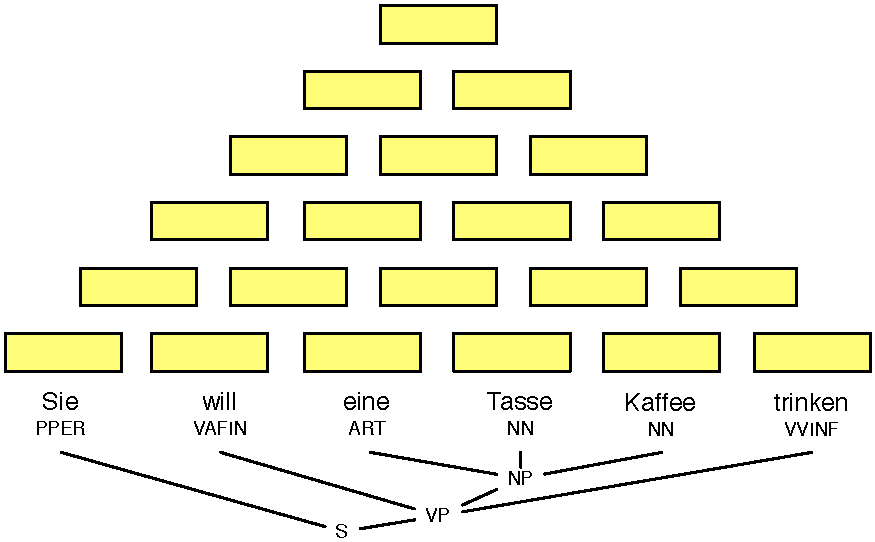
\includegraphics[scale=1]{chart-parsing-stacks.pdf}
\end{center}

%%%%%%%%%%%%%%%%%%%%%%%%%%%%%%%%%%%%%%%%%%%%%%%%%%%%%%%%%%%%%%%%%%%%%%%%%%%%

\slide{Syntax Decoding}
\vspace{-31mm}
\begin{center}
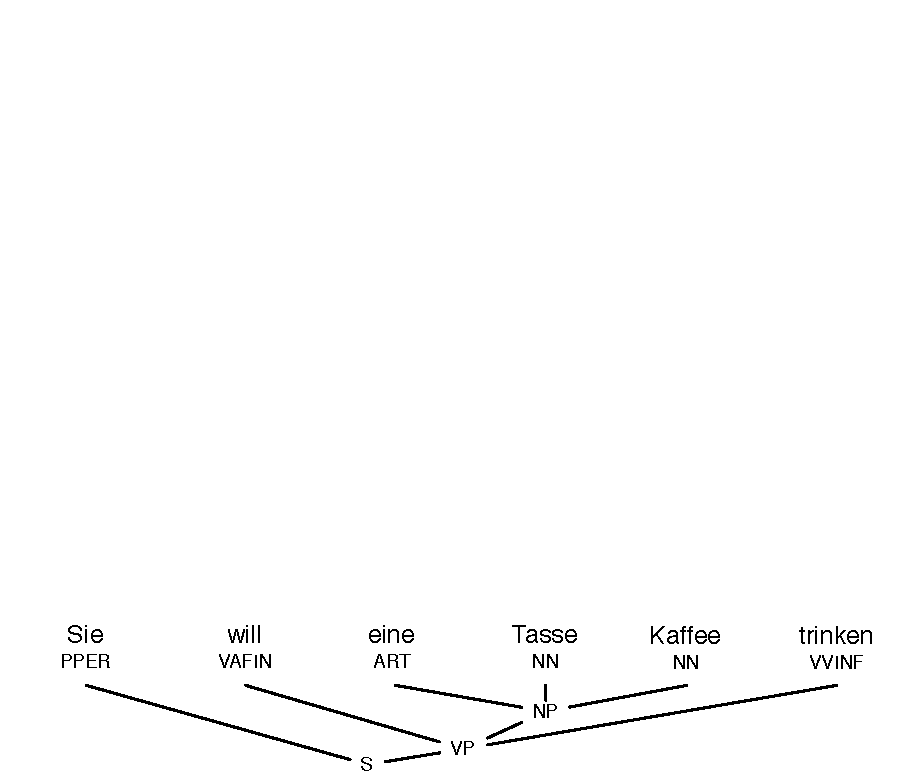
\includegraphics[scale=1.15]{chart-parsing0.pdf}\\
German input sentence with tree
\end{center}

%%%%%%%%%%%%%%%%%%%%%%%%%%%%%%%%%%%%%%%%%%%%%%%%%%%%%%%%%%%%%%%%%%%%%%%%%%%%

\slide{Syntax Decoding}
\vspace{-31mm}
\begin{center}
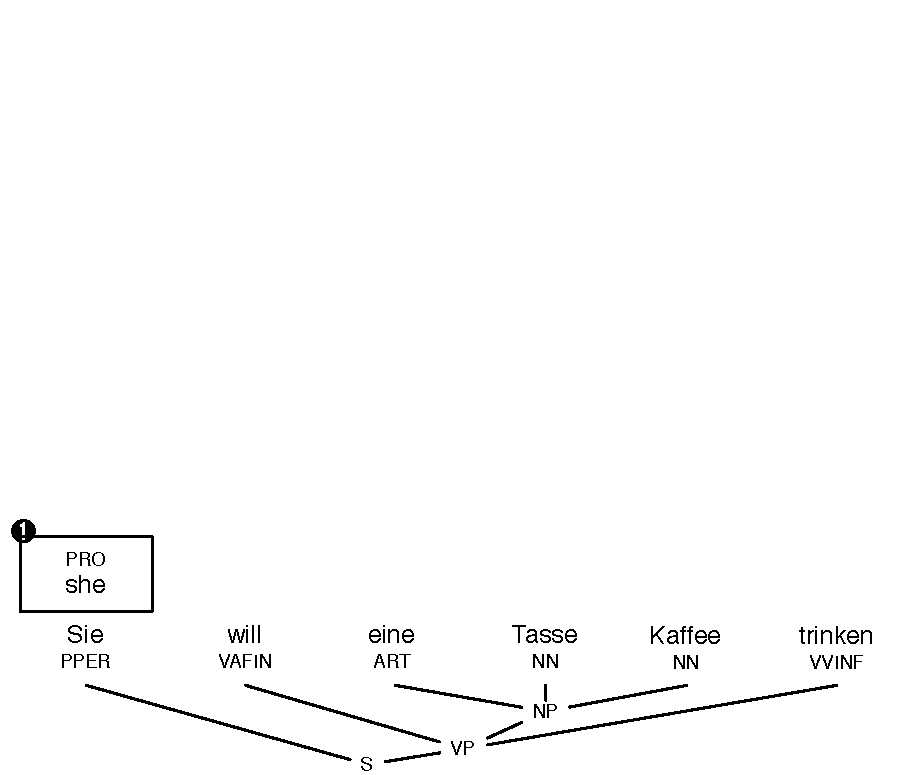
\includegraphics[scale=1.15]{chart-parsing1.pdf}\\
Purely lexical rule: filling a span with a translation (a constituent in the chart)
\end{center}

%%%%%%%%%%%%%%%%%%%%%%%%%%%%%%%%%%%%%%%%%%%%%%%%%%%%%%%%%%%%%%%%%%%%%%%%%%%%

\slide{Syntax Decoding}
\vspace{-31mm}
\begin{center}
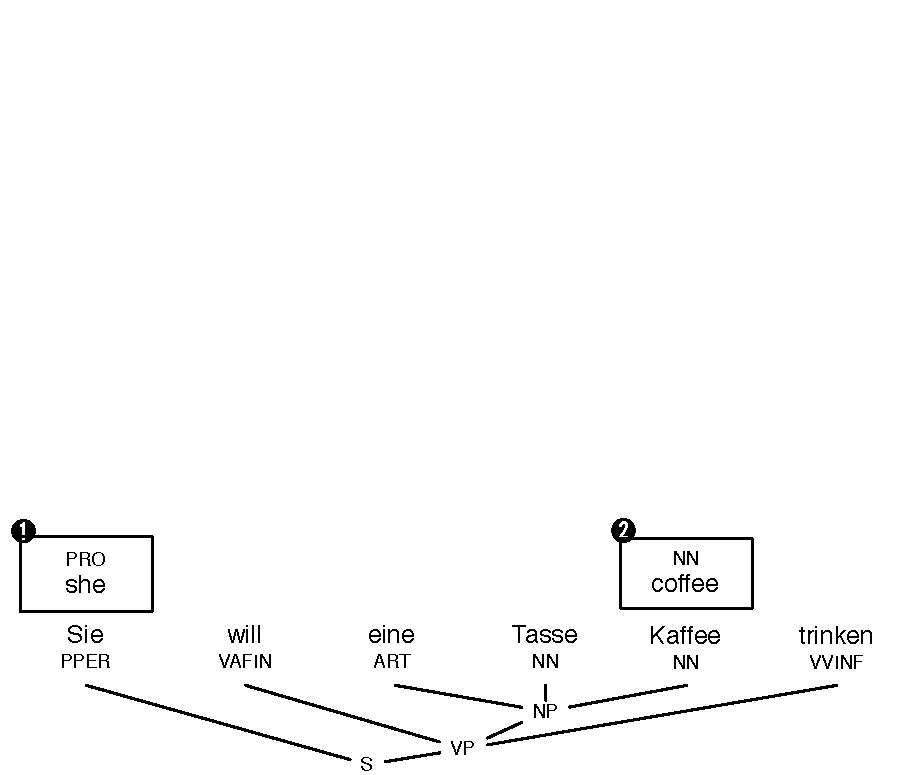
\includegraphics[scale=1.15]{chart-parsing2.pdf}\\
Purely lexical rule: filling a span with a translation (a constituent in the chart)
\end{center}

%%%%%%%%%%%%%%%%%%%%%%%%%%%%%%%%%%%%%%%%%%%%%%%%%%%%%%%%%%%%%%%%%%%%%%%%%%%%

\slide{Syntax Decoding}
\vspace{-31mm}
\begin{center}
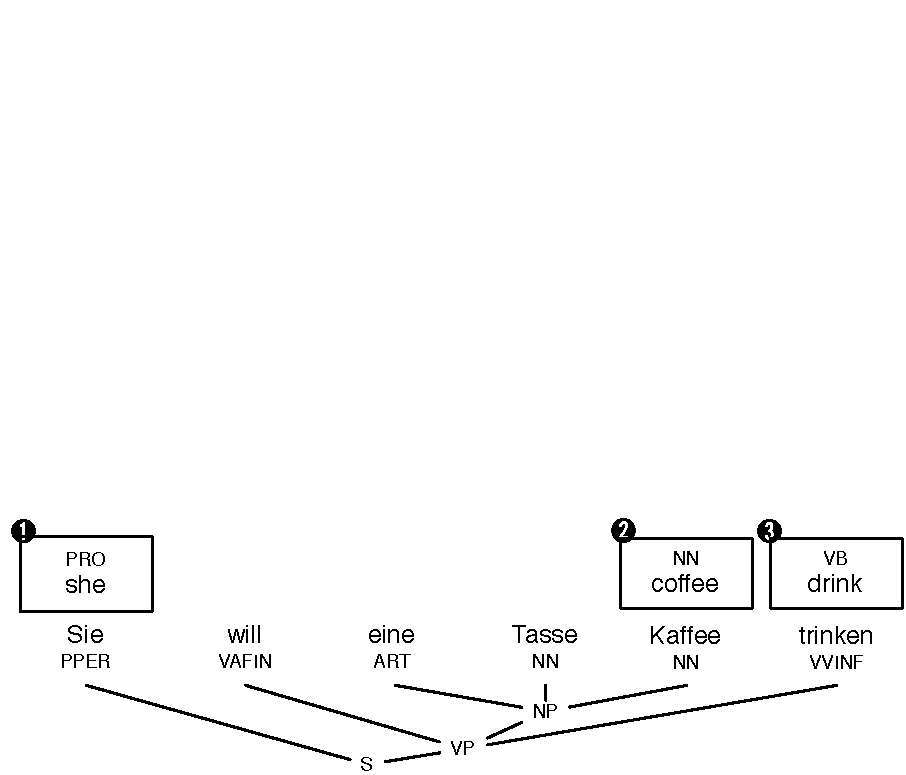
\includegraphics[scale=1.15]{chart-parsing3.pdf}\\
Purely lexical rule: filling a span with a translation (a constituent in the chart)
\end{center}

%%%%%%%%%%%%%%%%%%%%%%%%%%%%%%%%%%%%%%%%%%%%%%%%%%%%%%%%%%%%%%%%%%%%%%%%%%%%

\slide{Syntax Decoding}
\vspace{-31mm}
\begin{center}
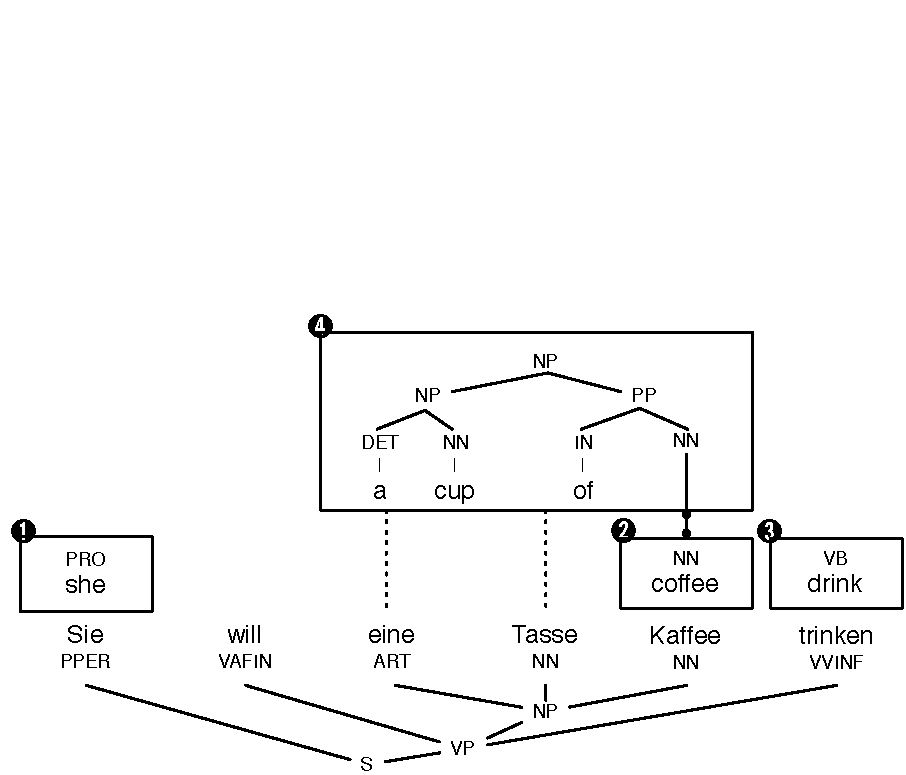
\includegraphics[scale=1.15]{chart-parsing4.pdf}\\
Complex rule: matching underlying constituent spans, and covering words
\end{center}

%%%%%%%%%%%%%%%%%%%%%%%%%%%%%%%%%%%%%%%%%%%%%%%%%%%%%%%%%%%%%%%%%%%%%%%%%%%%

\slide{Syntax Decoding}
\vspace{-31mm}
\begin{center}
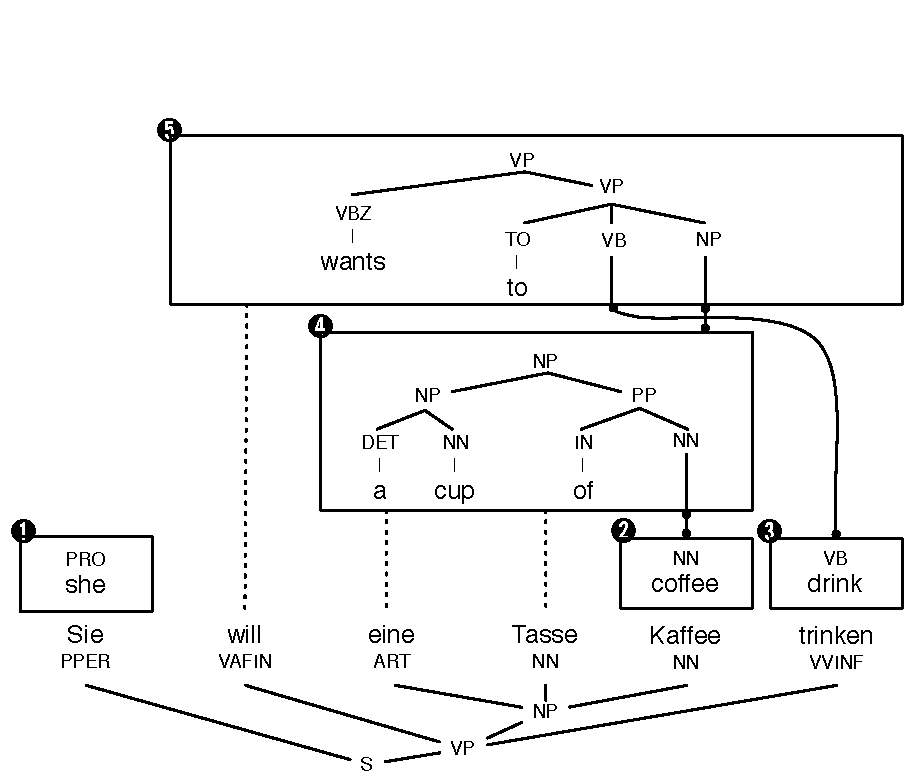
\includegraphics[scale=1.15]{chart-parsing5.pdf}\\
Complex rule with reordering
\end{center}

%%%%%%%%%%%%%%%%%%%%%%%%%%%%%%%%%%%%%%%%%%%%%%%%%%%%%%%%%%%%%%%%%%%%%%%%%%%%

\slide{Syntax Decoding}
\vspace{-31mm}
\begin{center}
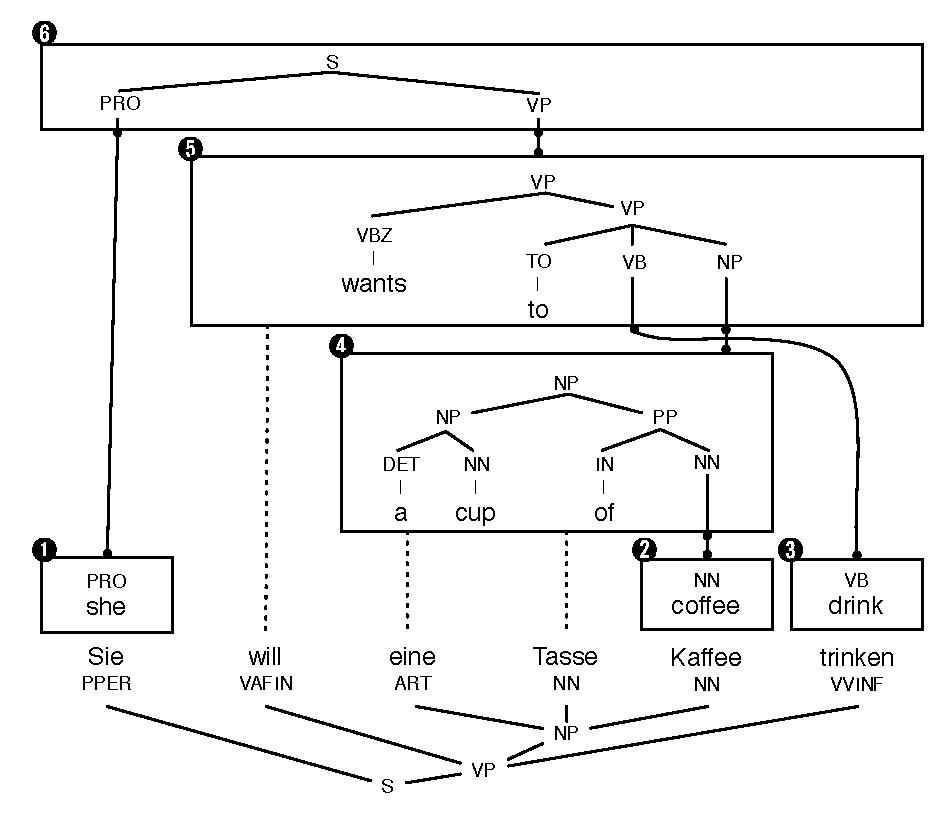
\includegraphics[scale=1.15]{chart-parsing.pdf}
\end{center}

%%%%%%%%%%%%%%%%%%%%%%%%%%%%%%%%%%%%%%%%%%%%%%%%%%%%%%%%%%%%%%%%%%%%%%%%%%%%

\slide{Bottom-Up Decoding}
\vspace{10mm}
\begin{itemize}
\item For each span, a stack of (partial) translations is maintained
\item Bottom-up: a higher stack is filled, once underlying stacks are complete
\begin{center} 
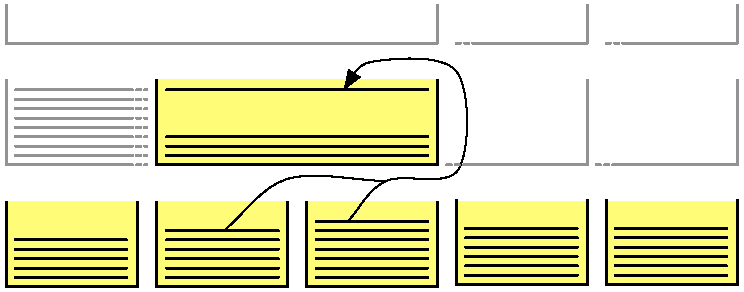
\includegraphics[scale=1.3]{chart-stacks-color.pdf}\\
\end{center}
\end{itemize}

%%%%%%%%%%%%%%%%%%%%%%%%%%%%%%%%%%%%%%%%%%%%%%%%%%%%%%%%%%%%%%%%%%%%%%%%%%%%

\slide{Naive Algorithm}
\vspace{15mm}
\begin{algorithmic}[1]
\renewcommand{\algorithmicrequire}{\textbf{Input:}} 
\renewcommand{\algorithmicensure}{\textbf{Output:}}
\REQUIRE Foreign sentence $\text{\bf f}=f_1,...f_{l_f}$, with syntax tree
\ENSURE English translation {\bf e}
\FORALL{spans [start,end] (bottom up)}
    \FORALL{sequences $s$ of hypotheses and words in span [start,end]}
      \FORALL{rules $r$}
        \IF{rule $r$ applies to chart sequence $s$}
          \STATE create new hypothesis $c$
          \STATE add hypothesis $c$ to chart
        \ENDIF
      \ENDFOR
    \ENDFOR
\ENDFOR 
\RETURN English translation {\bf e} from best hypothesis in span [0,$l_f$]
\end{algorithmic}

%%%%%%%%%%%%%%%%%%%%%%%%%%%%%%%%%%%%%%%%%%%%%%%%%%%%%%%%%%%%%%%%%%%%%%%%%%%%

\slide{Chart Organization}
\begin{center} \vspace{5mm}
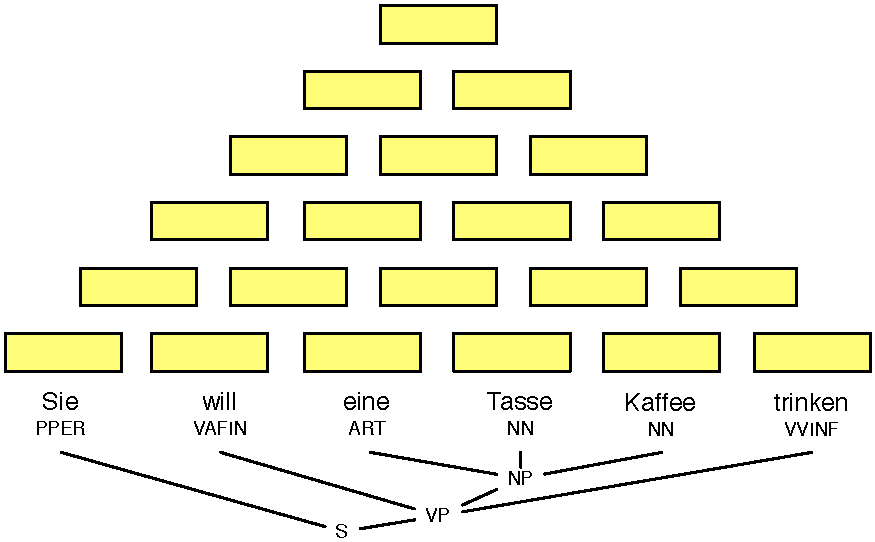
\includegraphics[scale=0.7]{chart-parsing-stacks.pdf} \hspace{10mm}
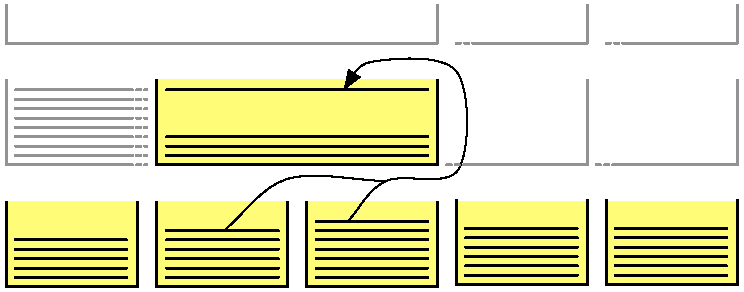
\includegraphics[scale=1]{chart-stacks-color.pdf}
\end{center}
\begin{itemize}
\item Chart consists of cells that cover contiguous spans over the input sentence
\item Each cell contains a set of hypotheses\footnote{In the book, they are called chart entries.}
\item Hypothesis = translation of span with target-side constituent
\end{itemize}

%%%%%%%%%%%%%%%%%%%%%%%%%%%%%%%%%%%%%%%%%%%%%%%%%%%%%%%%%%%%%%%%%%%%%%%%%%%%

\slide{Dynamic Programming}
\begin{center}\vspace{10mm}
Applying rule creates new hypothesis\\[15mm]
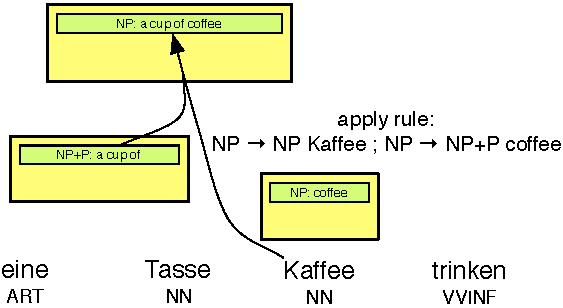
\includegraphics[scale=1.5]{chart-recombination.pdf}
\end{center}

%%%%%%%%%%%%%%%%%%%%%%%%%%%%%%%%%%%%%%%%%%%%%%%%%%%%%%%%%%%%%%%%%%%%%%%%%%%%

\slide{Dynamic Programming}
\begin{center}\vspace{5mm}
Another hypothesis\\[10mm]
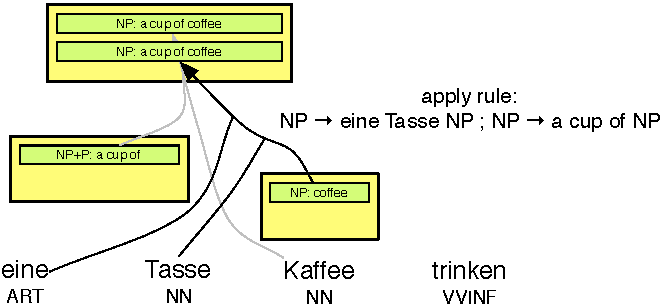
\includegraphics[scale=1.5]{chart-recombination2.pdf}\\[10mm]
Both hypotheses are indistiguishable in future search\\
$\rightarrow$ can be recombined
\end{center}

%%%%%%%%%%%%%%%%%%%%%%%%%%%%%%%%%%%%%%%%%%%%%%%%%%%%%%%%%%%%%%%%%%%%%%%%%%%%

\slide{Recombinable States}
\begin{center} \vspace{10mm}
Recombinable?\\[10mm]
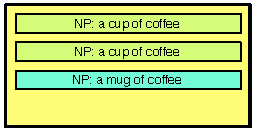
\includegraphics[scale=3]{chart-recombination3.pdf}
\end{center}

%%%%%%%%%%%%%%%%%%%%%%%%%%%%%%%%%%%%%%%%%%%%%%%%%%%%%%%%%%%%%%%%%%%%%%%%%%%%

\slide{Recombinable States}
\begin{center} \vspace{10mm}
Recombinable?\\[10mm]
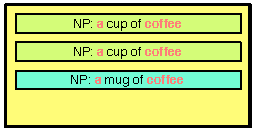
\includegraphics[scale=3]{chart-recombination4.pdf}\\[10mm]
Yes, iff max. 2-gram language model is used
\end{center}

%%%%%%%%%%%%%%%%%%%%%%%%%%%%%%%%%%%%%%%%%%%%%%%%%%%%%%%%%%%%%%%%%%%%%%%%%%%%

\slide{Recombinability}
\vspace{10mm}
Hypotheses have to match in
\begin{itemize} \itemsep -2mm
\item span of input words covered
\item output constituent label
\item first $n$--1 output words\\
\phantom{x} \hfill not properly scored, since they lack context
\item last $n$--1 output words\\
\phantom{x} \hfill still affect scoring of subsequently added words,\\ 
\phantom{x} \hfill just like in phrase-based decoding
\end{itemize}
\vspace{10mm}
\begin{center}
{\small ($n$ is the order of the n-gram language model)}
\end{center}

%%%%%%%%%%%%%%%%%%%%%%%%%%%%%%%%%%%%%%%%%%%%%%%%%%%%%%%%%%%%%%%%%%%%%%%%%%%%

\slide{Language Model Contexts}
\begin{center} \vspace{15mm}
When merging hypotheses, internal language model contexts are absorbed\\[15mm]
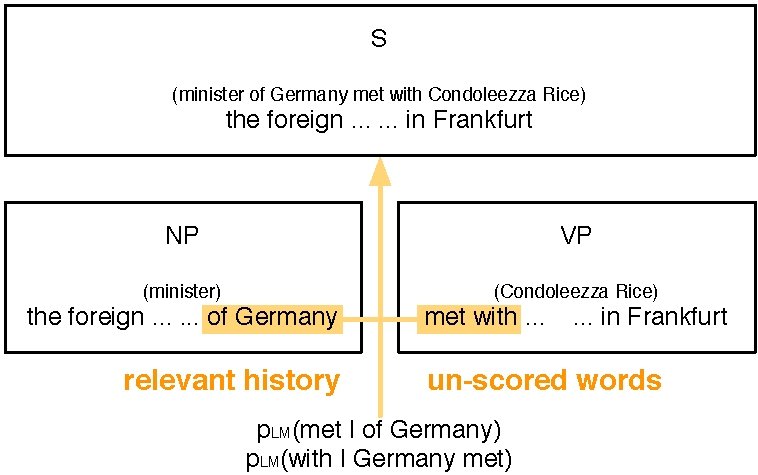
\includegraphics[scale=1.1]{syntax-rule-lm-merging.pdf}
\end{center} 

%%%%%%%%%%%%%%%%%%%%%%%%%%%%%%%%%%%%%%%%%%%%%%%%%%%%%%%%%%%%%%%%%%%%%%%%%%%%

\slide{Stack Pruning}
\begin{itemize}
\item Number of hypotheses in each chart cell explodes
\item[$\Rightarrow$] need to discard bad hypotheses\\ e.g., keep 100 best only
\item Different stacks for different output constituent labels?
\item Cost estimates
\begin{itemize}
\item translation model cost known
\item language model cost for internal words known\\
$\rightarrow$ estimates for initial words
\item outside cost estimate?\\
(how useful will be a NP covering input words 3--5 later on?)
\end{itemize}
\end{itemize}

%%%%%%%%%%%%%%%%%%%%%%%%%%%%%%%%%%%%%%%%%%%%%%%%%%%%%%%%%%%%%%%%%%%%%%%%%%%%

\slide{Naive Algorithm: Blow-ups}
\begin{itemize}
\item Many subspan sequences
\begin{center}
{\bf for all} sequences $s$ of hypotheses and words in span [start,end]
\end{center}
\item Many rules
\begin{center}
{\bf for all} {rules $r$}
\end{center}
\item Checking if a rule applies not trivial
\begin{center}
rule $r$ applies to chart sequence $s$
\end{center}
\item[$\Rightarrow$] Unworkable
\end{itemize}

%%%%%%%%%%%%%%%%%%%%%%%%%%%%%%%%%%%%%%%%%%%%%%%%%%%%%%%%%%%%%%%%%%%%%%%%%%%%

\slide{Solution}
\vspace{30mm}
\begin{itemize}\itemsep 10mm
\item Prefix tree data structure for rules
\item Dotted rules
\item Cube pruning
\end{itemize}

%%%%%%%%%%%%%%%%%%%%%%%%%%%%%%%%%%%%%%%%%%%%%%%%%%%%%%%%%%%%%%%%%%%%%%%%%%%%

\slide{Storing Rules}
\begin{itemize}
\item First concern: do they apply to span?\\
$\rightarrow$ have to match available hypotheses and input words
\item Example rule
\begin{center}
\example{{\sc np} $\rightarrow$ 
$\text{\sc x}_1$ des $\text{\sc x}_2$ $\;|\;$
$\text{\sc np}_1$ of the $\text{\sc nn}_2$}
\end{center}
\item Check for applicability
\begin{itemize}
\item is there an initial sub-span that with a hypothesis with constituent label \example{\sc np}?
\item is it followed by a sub-span over the word \example{des}?
\item is it followed by a final sub-span with a hypothesis with  label \example{\sc nn}?
\end{itemize}
\item Sequence of relevant information
\begin{center}
\example{\sc np} $\bullet$ \example{des}  $\bullet$ \example{\sc nn}  $\bullet$ \example{$\text{\sc np}_1$ of the $\text{\sc nn}_2$}
\end{center}
\end{itemize}


%%%%%%%%%%%%%%%%%%%%%%%%%%%%%%%%%%%%%%%%%%%%%%%%%%%%%%%%%%%%%%%%%%%%%%%%%%%%

\slide{Rule Applicability Check}
\vspace{20mm}
\begin{center}
Trying to cover a span of six words with given rule\\[20mm]
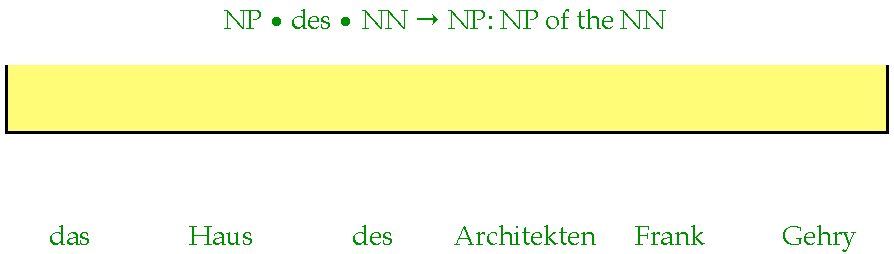
\includegraphics[scale=1.6]{rule-lookup1.pdf}
\end{center}

%%%%%%%%%%%%%%%%%%%%%%%%%%%%%%%%%%%%%%%%%%%%%%%%%%%%%%%%%%%%%%%%%%%%%%%%%%%%

\slide{Rule Applicability Check}
\vspace{20mm}
\begin{center}
First: check for hypotheses with output constituent label \example{\sc np}\\[20mm]
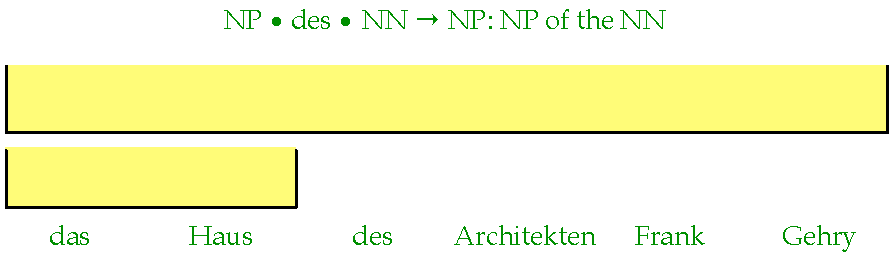
\includegraphics[scale=1.6]{rule-lookup2.pdf}
\end{center}

%%%%%%%%%%%%%%%%%%%%%%%%%%%%%%%%%%%%%%%%%%%%%%%%%%%%%%%%%%%%%%%%%%%%%%%%%%%%

\slide{Rule Applicability Check}
\vspace{20mm}
\begin{center}
Found \example{\sc np} hypothesis in cell, matched first symbol of rule\\[20mm]
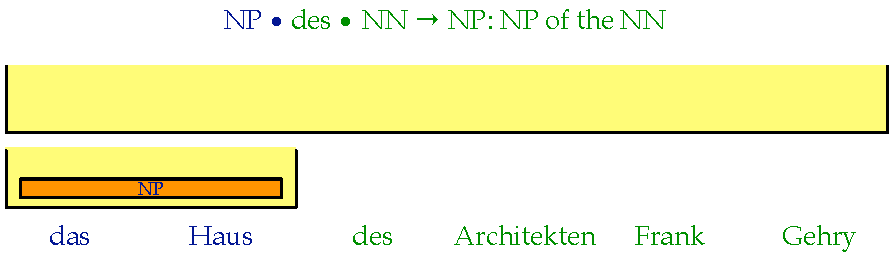
\includegraphics[scale=1.6]{rule-lookup3.pdf}
\end{center}

%%%%%%%%%%%%%%%%%%%%%%%%%%%%%%%%%%%%%%%%%%%%%%%%%%%%%%%%%%%%%%%%%%%%%%%%%%%%

\slide{Rule Applicability Check}
\vspace{20mm}
\begin{center}
Matched word \example{des}, matched second symbol of rule\\[20mm]
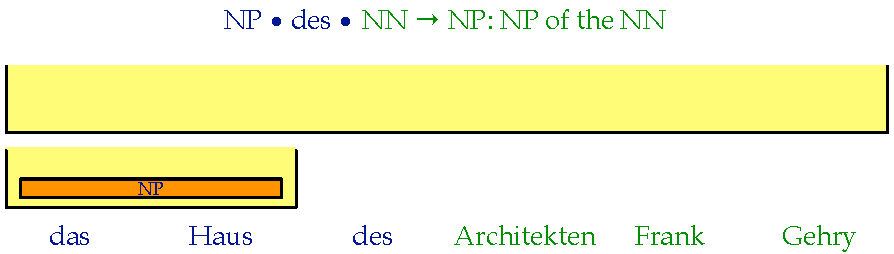
\includegraphics[scale=1.6]{rule-lookup4.pdf}
\end{center}

%%%%%%%%%%%%%%%%%%%%%%%%%%%%%%%%%%%%%%%%%%%%%%%%%%%%%%%%%%%%%%%%%%%%%%%%%%%%

\slide{Rule Applicability Check}
\vspace{20mm}
\begin{center}
Found a \example{\sc nn} hypothesis in cell, matched last symbol of rule\\[20mm]
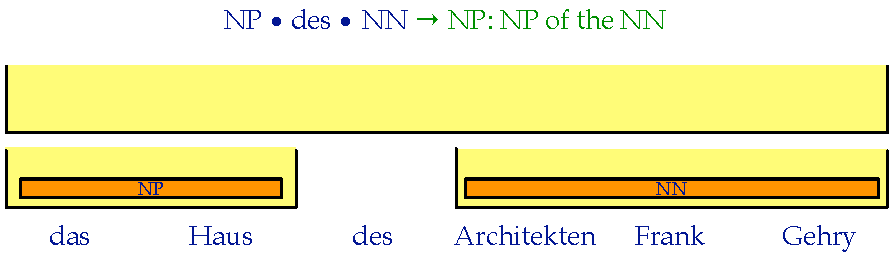
\includegraphics[scale=1.6]{rule-lookup5.pdf}
\end{center}

%%%%%%%%%%%%%%%%%%%%%%%%%%%%%%%%%%%%%%%%%%%%%%%%%%%%%%%%%%%%%%%%%%%%%%%%%%%%

\slide{Rule Applicability Check}
\vspace{20mm}
\begin{center}
Matched entire rule $\rightarrow$ apply to create a \example{\sc np} hypothesis\\[20mm]
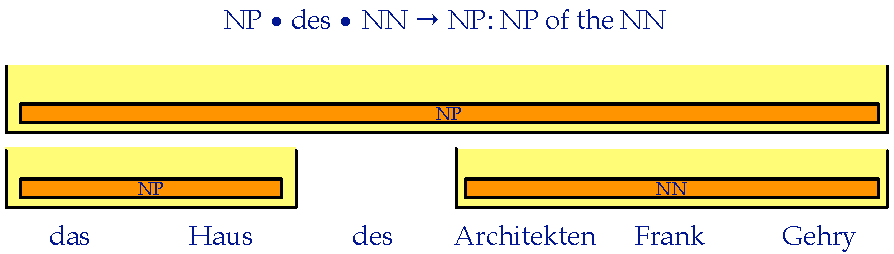
\includegraphics[scale=1.6]{rule-lookup6.pdf}
\end{center}

%%%%%%%%%%%%%%%%%%%%%%%%%%%%%%%%%%%%%%%%%%%%%%%%%%%%%%%%%%%%%%%%%%%%%%%%%%%%

\slide{Rule Applicability Check}
\vspace{16mm}
\begin{center}
Look up output words to create new hypothesis\\
(note: there may be many matching underlying \example{\sc np} and \example{\sc nn} hypotheses)\\[15mm]
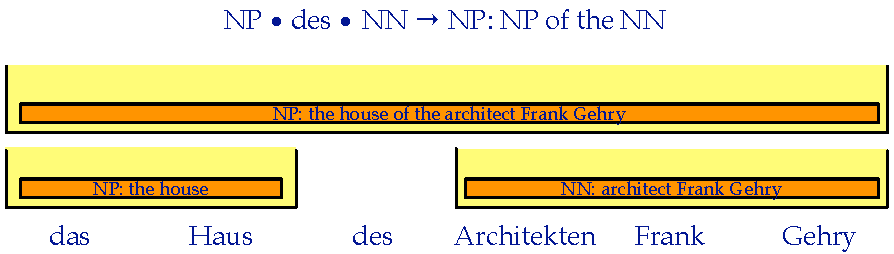
\includegraphics[scale=1.6]{rule-lookup.pdf}
\end{center}

%%%%%%%%%%%%%%%%%%%%%%%%%%%%%%%%%%%%%%%%%%%%%%%%%%%%%%%%%%%%%%%%%%%%%%%%%%%%

\slide{Checking Rules vs. Finding Rules}
\vspace{20mm}
\begin{itemize}
\item What we showed:
\begin{itemize}
\item given a rule
\item check if and how it can be applied
\end{itemize}
\item But there are too many rules (millions) to check them all
\item Instead:
\begin{itemize}
\item given the underlying chart cells and input words
\item find which rules apply
\end{itemize}
\end{itemize}

%%%%%%%%%%%%%%%%%%%%%%%%%%%%%%%%%%%%%%%%%%%%%%%%%%%%%%%%%%%%%%%%%%%%%%%%%%%%

\slide{Prefix Tree for Rules}
\begin{center}
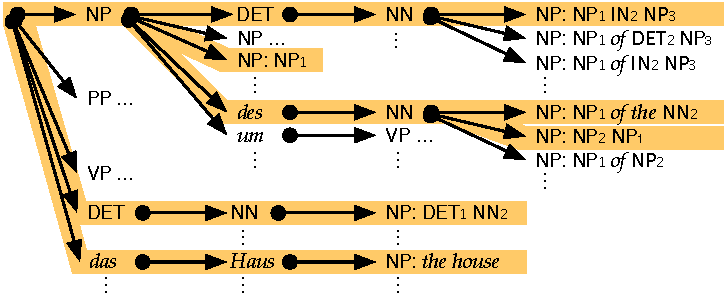
\includegraphics[scale=1.4]{accessing-grammar-rules-prefix.pdf}\\[2mm]
{\bf Highlighted Rules}\\
\example{
{\sc np} $\rightarrow$ 
$\text{\sc np}_1$ $\text{\sc det}_2$ $\text{\sc nn}_3$ $\;|\;$
$\text{\sc np}_1$ $\text{\sc in}_2$ $\text{\sc nn}_3$ \\
{\sc np} $\rightarrow$ 
$\text{\sc np}_1$ $\;|\;$
$\text{\sc np}_1$ \\
{\sc np} $\rightarrow$ 
$\text{\sc np}_1$ des $\text{\sc nn}_2$ $\;|\;$
$\text{\sc np}_1$ of the $\text{\sc nn}_2$ \\
{\sc np} $\rightarrow$ 
$\text{\sc np}_1$ des $\text{\sc nn}_2$ $\;|\;$
$\text{\sc np}_2$ $\text{\sc np}_1$ \\
{\sc np} $\rightarrow$ 
$\text{\sc det}_1$ $\text{\sc nn}_2$ $\;|\;$
$\text{\sc det}_1$ $\text{\sc nn}_2$ \\
{\sc np} $\rightarrow$ 
das Haus $\;|\;$
the house}
\end{center}

%%%%%%%%%%%%%%%%%%%%%%%%%%%%%%%%%%%%%%%%%%%%%%%%%%%%%%%%%%%%%%%%%%%%%%%%%%%%

\slide{Dotted Rules: Key Insight}
\vspace{10mm}
\begin{itemize}\itemsep 10mm
\item If we can apply a rule like
\begin{center}\vspace{-5mm}
\example{p $\rightarrow$ A B C $\;|\;$ x}
\end{center}\vspace{-5mm}
to a span
\item Then we could have applied a rule like
\begin{center}\vspace{-5mm}
\example{q $\rightarrow$ A B $\;|\;$ y}
\end{center}\vspace{-5mm}
to a sub-span with the same starting word
\item[$\Rightarrow$] We can re-use rule lookup by storing \example{A B $\bullet$} (dotted rule)
\end{itemize}

%%%%%%%%%%%%%%%%%%%%%%%%%%%%%%%%%%%%%%%%%%%%%%%%%%%%%%%%%%%%%%%%%%%%%%%%%%%%

\slide{Finding Applicable Rules in Prefix Tree}
\begin{center}\vspace{55mm}
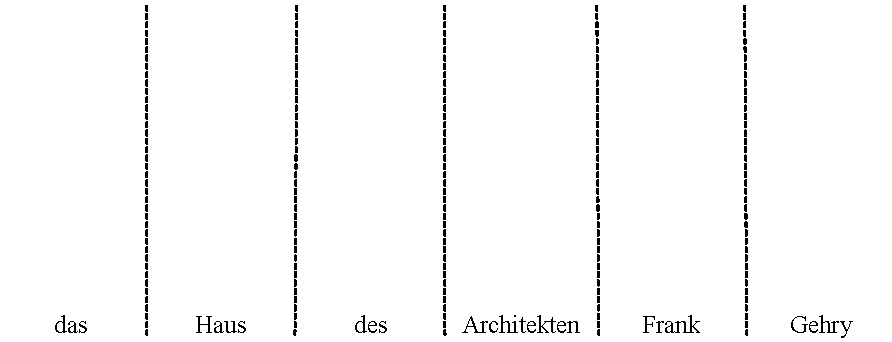
\includegraphics[scale=1.4]{accessing-grammar-rules-early-example00.pdf}
\end{center}

%%%%%%%%%%%%%%%%%%%%%%%%%%%%%%%%%%%%%%%%%%%%%%%%%%%%%%%%%%%%%%%%%%%%%%%%%%%%

\slide{Covering the First Cell}
\begin{center}\vspace{55mm}
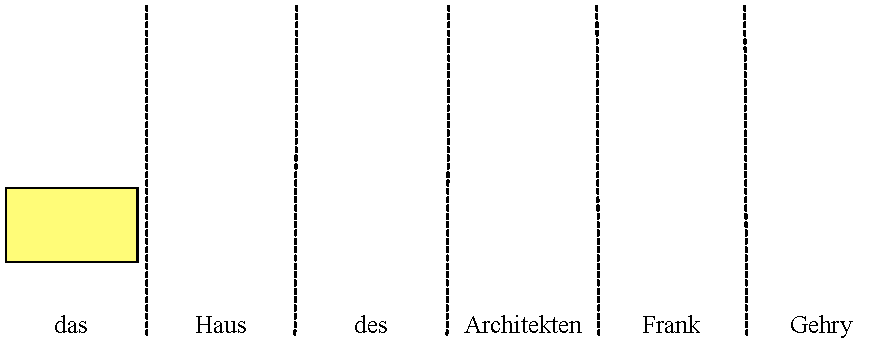
\includegraphics[scale=1.4]{accessing-grammar-rules-early-example0.pdf}
\end{center}

%%%%%%%%%%%%%%%%%%%%%%%%%%%%%%%%%%%%%%%%%%%%%%%%%%%%%%%%%%%%%%%%%%%%%%%%%%%%

\slide{Looking up Rules in the Prefix Tree}
\begin{center}\vspace{15mm}

\includegraphics[scale=1.4]{accessing-grammar-rules-prefix-early0.pdf}\\[31mm]
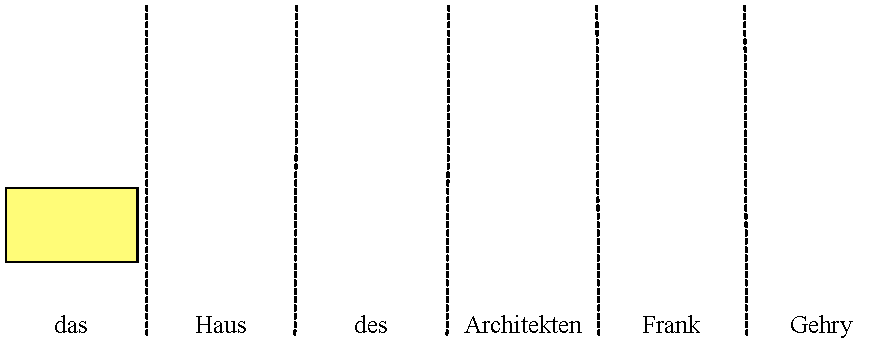
\includegraphics[scale=1.4]{accessing-grammar-rules-early-example0.pdf}
\end{center}

%%%%%%%%%%%%%%%%%%%%%%%%%%%%%%%%%%%%%%%%%%%%%%%%%%%%%%%%%%%%%%%%%%%%%%%%%%%%

\slide{Taking Note of the Dotted Rule}
\begin{center}\vspace{15mm}

\includegraphics[scale=1.4]{accessing-grammar-rules-prefix-early0.pdf}\\[31mm]
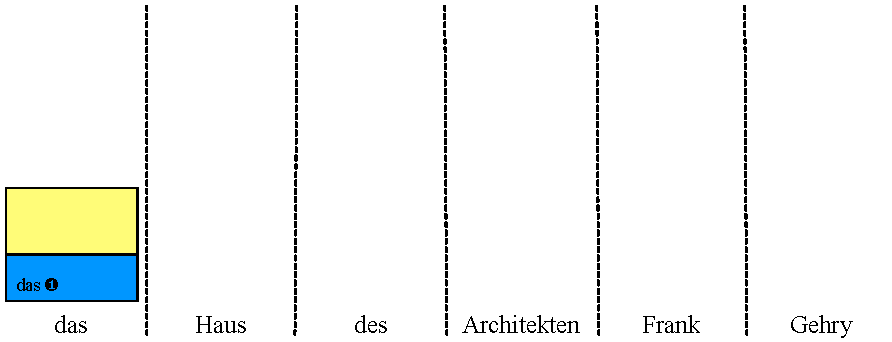
\includegraphics[scale=1.4]{accessing-grammar-rules-early-example1.pdf}
\end{center}

%%%%%%%%%%%%%%%%%%%%%%%%%%%%%%%%%%%%%%%%%%%%%%%%%%%%%%%%%%%%%%%%%%%%%%%%%%%%

\slide{Checking if Dotted Rule has Translations}
\begin{center}\vspace{15mm}
\includegraphics[scale=1.4]{accessing-grammar-rules-prefix-early1.pdf}\\[27mm]
\includegraphics[scale=1.4]{accessing-grammar-rules-early-example1.pdf}
\end{center}

%%%%%%%%%%%%%%%%%%%%%%%%%%%%%%%%%%%%%%%%%%%%%%%%%%%%%%%%%%%%%%%%%%%%%%%%%%%%

\slide{Applying the Translation Rules}
\begin{center}\vspace{15mm}
\includegraphics[scale=1.4]{accessing-grammar-rules-prefix-early1.pdf}\\[27mm]
\includegraphics[scale=1.4]{accessing-grammar-rules-early-example2.pdf}
\end{center}

%%%%%%%%%%%%%%%%%%%%%%%%%%%%%%%%%%%%%%%%%%%%%%%%%%%%%%%%%%%%%%%%%%%%%%%%%%%%

\slide{Looking up Constituent Label in Prefix Tree}
\begin{center}\vspace{13mm}
\includegraphics[scale=1.4]{accessing-grammar-rules-prefix-early2.pdf}\\[22mm]
\includegraphics[scale=1.4]{accessing-grammar-rules-early-example2.pdf}
\end{center}

%%%%%%%%%%%%%%%%%%%%%%%%%%%%%%%%%%%%%%%%%%%%%%%%%%%%%%%%%%%%%%%%%%%%%%%%%%%%

\slide{Add to Span's List of Dotted Rules}
\begin{center}\vspace{14mm}
\includegraphics[scale=1.4]{accessing-grammar-rules-prefix-early2.pdf}\\[22mm]
\includegraphics[scale=1.4]{accessing-grammar-rules-early-example3.pdf}
\end{center}

%%%%%%%%%%%%%%%%%%%%%%%%%%%%%%%%%%%%%%%%%%%%%%%%%%%%%%%%%%%%%%%%%%%%%%%%%%%%

\slide{Moving on to the Next Cell}
\begin{center}\vspace{7mm}
\includegraphics[scale=1.4]{accessing-grammar-rules-prefix-early2.pdf}\\[29mm]
\includegraphics[scale=1.4]{accessing-grammar-rules-early-example4.pdf}
\end{center}

%%%%%%%%%%%%%%%%%%%%%%%%%%%%%%%%%%%%%%%%%%%%%%%%%%%%%%%%%%%%%%%%%%%%%%%%%%%%

\slide{Looking up Rules in the Prefix Tree}
\begin{center}\vspace{7mm}
\includegraphics[scale=1.4]{accessing-grammar-rules-prefix-early3.pdf}\\[19mm]
\includegraphics[scale=1.4]{accessing-grammar-rules-early-example4.pdf}
\end{center}

%%%%%%%%%%%%%%%%%%%%%%%%%%%%%%%%%%%%%%%%%%%%%%%%%%%%%%%%%%%%%%%%%%%%%%%%%%%%

\slide{Taking Note of the Dotted Rule}
\begin{center}\vspace{7mm}
\includegraphics[scale=1.4]{accessing-grammar-rules-prefix-early3.pdf}\\[19mm]
\includegraphics[scale=1.4]{accessing-grammar-rules-early-example5.pdf}
\end{center}

%%%%%%%%%%%%%%%%%%%%%%%%%%%%%%%%%%%%%%%%%%%%%%%%%%%%%%%%%%%%%%%%%%%%%%%%%%%%

\slide{Checking if Dotted Rule has Translations}
\begin{center}\vspace{7mm}
\includegraphics[scale=1.4]{accessing-grammar-rules-prefix-early4.pdf}\\[8mm]
\includegraphics[scale=1.4]{accessing-grammar-rules-early-example5.pdf}
\end{center}

%%%%%%%%%%%%%%%%%%%%%%%%%%%%%%%%%%%%%%%%%%%%%%%%%%%%%%%%%%%%%%%%%%%%%%%%%%%%

\slide{Applying the Translation Rules}
\begin{center}\vspace{7mm}
\includegraphics[scale=1.4]{accessing-grammar-rules-prefix-early4.pdf}\\[8mm]
\includegraphics[scale=1.4]{accessing-grammar-rules-early-example6.pdf}
\end{center}

%%%%%%%%%%%%%%%%%%%%%%%%%%%%%%%%%%%%%%%%%%%%%%%%%%%%%%%%%%%%%%%%%%%%%%%%%%%%

\slide{Looking up Constituent Label in Prefix Tree}
\begin{center}\vspace{7mm}
\includegraphics[scale=1.4]{accessing-grammar-rules-prefix-early5.pdf}\\[-1mm]
\includegraphics[scale=1.4]{accessing-grammar-rules-early-example6.pdf}
\end{center}

%%%%%%%%%%%%%%%%%%%%%%%%%%%%%%%%%%%%%%%%%%%%%%%%%%%%%%%%%%%%%%%%%%%%%%%%%%%%

\slide{Add to Span's List of Dotted Rules}
\begin{center}\vspace{7mm}
\includegraphics[scale=1.4]{accessing-grammar-rules-prefix-early5.pdf}\\[-1mm]
\includegraphics[scale=1.4]{accessing-grammar-rules-early-example7.pdf}
\end{center}

%%%%%%%%%%%%%%%%%%%%%%%%%%%%%%%%%%%%%%%%%%%%%%%%%%%%%%%%%%%%%%%%%%%%%%%%%%%%

\slide{More of the Same}
\begin{center}\vspace{9mm}
\includegraphics[scale=1.4]{accessing-grammar-rules-prefix-early5.pdf}\\[-1mm]
\includegraphics[scale=1.4]{accessing-grammar-rules-early-example8.pdf}
\end{center}

%%%%%%%%%%%%%%%%%%%%%%%%%%%%%%%%%%%%%%%%%%%%%%%%%%%%%%%%%%%%%%%%%%%%%%%%%%%%

\slide{Moving on to the Next Cell}
\begin{center}\vspace{7mm}
\includegraphics[scale=1.4]{accessing-grammar-rules-prefix-early5.pdf}\\[-1mm]
\includegraphics[scale=1.4]{accessing-grammar-rules-early-example9.pdf}
\end{center}

%%%%%%%%%%%%%%%%%%%%%%%%%%%%%%%%%%%%%%%%%%%%%%%%%%%%%%%%%%%%%%%%%%%%%%%%%%%%

\slide{Covering a Longer Span}
\begin{center}\vspace{8mm}
Cannot consume multiple words at once\\[2mm]
All rules are extensions of existing dotted rules\\[2mm]
Here: only extensions of span over \example{das} possible\\[17mm]
\includegraphics[scale=1.4]{accessing-grammar-rules-early-example9.pdf}
\end{center}

%%%%%%%%%%%%%%%%%%%%%%%%%%%%%%%%%%%%%%%%%%%%%%%%%%%%%%%%%%%%%%%%%%%%%%%%%%%%

\slide{Extensions of Span over \example{das}}
\begin{center}\vspace{7mm}
\includegraphics[scale=1.4]{accessing-grammar-rules-prefix-early6.pdf}\\[-1mm]
\includegraphics[scale=1.4]{accessing-grammar-rules-early-example9.pdf}
\end{center}

%%%%%%%%%%%%%%%%%%%%%%%%%%%%%%%%%%%%%%%%%%%%%%%%%%%%%%%%%%%%%%%%%%%%%%%%%%%%

\slide{Looking up Rules in the Prefix Tree}
\begin{center}\vspace{7mm}
\includegraphics[scale=1.4]{accessing-grammar-rules-prefix-early7.pdf}\\[9mm]
\includegraphics[scale=1.4]{accessing-grammar-rules-early-example9.pdf}
\end{center}

%%%%%%%%%%%%%%%%%%%%%%%%%%%%%%%%%%%%%%%%%%%%%%%%%%%%%%%%%%%%%%%%%%%%%%%%%%%%

\slide{Taking Note of the Dotted Rule}
\begin{center}\vspace{7mm}
\includegraphics[scale=1.4]{accessing-grammar-rules-prefix-early7.pdf}\\[9mm]
\includegraphics[scale=1.4]{accessing-grammar-rules-early-example10.pdf}
\end{center}

%%%%%%%%%%%%%%%%%%%%%%%%%%%%%%%%%%%%%%%%%%%%%%%%%%%%%%%%%%%%%%%%%%%%%%%%%%%%

\slide{Checking if Dotted Rules have Translations}
\begin{center}\vspace{7mm}
\includegraphics[scale=1.4]{accessing-grammar-rules-prefix-early8.pdf}\\[9mm]
\includegraphics[scale=1.4]{accessing-grammar-rules-early-example10.pdf}
\end{center}

%%%%%%%%%%%%%%%%%%%%%%%%%%%%%%%%%%%%%%%%%%%%%%%%%%%%%%%%%%%%%%%%%%%%%%%%%%%%

\slide{Applying the Translation Rules}
\begin{center}\vspace{7mm}
\includegraphics[scale=1.4]{accessing-grammar-rules-prefix-early8.pdf}\\[9mm]
\includegraphics[scale=1.4]{accessing-grammar-rules-early-example11.pdf}
\end{center}

%%%%%%%%%%%%%%%%%%%%%%%%%%%%%%%%%%%%%%%%%%%%%%%%%%%%%%%%%%%%%%%%%%%%%%%%%%%%

\slide{Looking up Constituent Label in Prefix Tree}
\begin{center}\vspace{7mm}
\includegraphics[scale=1.4]{accessing-grammar-rules-prefix-early9.pdf}\\[-1mm]
\includegraphics[scale=1.4]{accessing-grammar-rules-early-example11.pdf}
\end{center}

%%%%%%%%%%%%%%%%%%%%%%%%%%%%%%%%%%%%%%%%%%%%%%%%%%%%%%%%%%%%%%%%%%%%%%%%%%%%

\slide{Add to Span's List of Dotted Rules}
\begin{center}\vspace{7mm}
\includegraphics[scale=1.4]{accessing-grammar-rules-prefix-early9.pdf}\\[-1mm]
\includegraphics[scale=1.4]{accessing-grammar-rules-early-example12.pdf}
\end{center}

%%%%%%%%%%%%%%%%%%%%%%%%%%%%%%%%%%%%%%%%%%%%%%%%%%%%%%%%%%%%%%%%%%%%%%%%%%%%

\slide{Even Larger Spans}
\begin{center}\vspace{5mm}
Extend lists of dotted rules with cell constituent labels\\[5mm]
span's dotted rule list (with same start)\\ plus neighboring\\ span's constituent labels of hypotheses (with same end)\\[5mm]
\includegraphics[scale=1.4]{accessing-grammar-rules-early-example14.pdf}
\end{center}

%%%%%%%%%%%%%%%%%%%%%%%%%%%%%%%%%%%%%%%%%%%%%%%%%%%%%%%%%%%%%%%%%%%%%%%%%%%%

\slide{Reflections}
\vspace{20mm}
\begin{itemize}\itemsep 10mm
\item Complexity \maths{$O(rn^3)$} with sentence length \maths{$n$} and size of dotted rule list \maths{$r$}
\begin{itemize}
\item may introduce maximum size for spans that do not start at beginning
\item may limit size of dotted rule list (very arbitrary)
\end{itemize}
\item Does the list of dotted rules explode?
\item Yes, if there are many rules with neighboring target-side non-terminals
\begin{itemize}
\item such rules apply in many places
\item rules with words are much more restricted
\end{itemize}
\end{itemize}

%%%%%%%%%%%%%%%%%%%%%%%%%%%%%%%%%%%%%%%%%%%%%%%%%%%%%%%%%%%%%%%%%%%%%%%%%%%%

\slide{Difficult Rules}
\begin{itemize}
\item Some rules may apply in too many ways
\item Neighboring input non-terminals
\begin{center}
\example{{\sc vp} $\rightarrow$ gibt $\text{\sc x}_1$ $\text{\sc x}_2$ $|$ gives $\text{\sc np}_2$ to $\text{\sc np}_1$}
\end{center}
\begin{itemize}
\item non-terminals may match many different pairs of spans
\item especially a problem for hierarchical models (no constituent label restrictions) 
\item may be okay for syntax-models
\end{itemize}
\item Three neighboring input non-terminals
\begin{center}
\example{{\sc vp} $\rightarrow$ trifft $\text{\sc x}_1$ $\text{\sc x}_2$  $\text{\sc x}_3$ heute $|$ meets $\text{\sc np}_1$ today $\text{\sc pp}_2$ $\text{\sc pp}_3$}
\end{center}
\begin{itemize}
\item will get out of hand even for syntax models
\end{itemize}

%examples
%neighboring non-terminals
%DeNero
%Hopkins
%Asynchronous binarization?
\end{itemize}

%%%%%%%%%%%%%%%%%%%%%%%%%%%%%%%%%%%%%%%%%%%%%%%%%%%%%%%%%%%%%%%%%%%%%%%%%%%%

\slide{Where are we now?}
\vspace{20mm}
\begin{itemize}\itemsep 5mm
\item We know which rules apply
\item We know where they apply (each non-terminal tied to a span)
\item But there are still many choices
\begin{itemize}
\item many possible translations
\item each non-terminal may match multiple hypotheses
\item[$\rightarrow$] number choices exponential with number of non-terminals
\end{itemize}
\end{itemize}

%%%%%%%%%%%%%%%%%%%%%%%%%%%%%%%%%%%%%%%%%%%%%%%%%%%%%%%%%%%%%%%%%%%%%%%%%%%%

\slide{Rules with One Non-Terminal}
\vspace{5mm}
\begin{center}
Found applicable rules \example{{\sc pp} $\rightarrow$ des {\sc x} $|$ ... {\sc np} ...}\\[5mm]
\includegraphics[scale=1.5]{cube-pruning-lexrule.pdf}
\end{center}
\begin{itemize} \itemsep -3mm
\item Non-terminal will be filled any of \maths{$h$} underlying matching hypotheses
\item Choice of \maths{$t$} lexical translations 
\item[$\Rightarrow$] Complexity \maths{$O(ht)$}
\end{itemize}
\begin{center}
{\small (note: we may not group rules by target constituent label,\\ so a rule \example{{\sc np} $\rightarrow$ des {\sc x} $|$ the {\sc np}} would also be considered here as well)}
\end{center}

%%%%%%%%%%%%%%%%%%%%%%%%%%%%%%%%%%%%%%%%%%%%%%%%%%%%%%%%%%%%%%%%%%%%%%%%%%%%

\slide{Rules with Two Non-Terminals}
\vspace{5mm}
\begin{center}
Found applicable rule \example{{\sc np} $\rightarrow$ $\text{\sc x}_1$ des $\text{\sc x}_2$ $|$ $\text{\sc np}_1$ ... $\text{\sc np}_2$}\\[5mm]
\includegraphics[scale=1.5]{cube-pruning-3.pdf}
\end{center}
\begin{itemize} \itemsep -3mm
\item Two non-terminal will be filled any of \maths{$h$} underlying matching hypotheses each
\item Choice of \maths{$t$} lexical translations 
\item[$\Rightarrow$] Complexity \maths{$O(h^2t)$} --- a three-dimensional "cube" of choices
\end{itemize}
\vspace{5mm}
\begin{center}
{\small (note: rules may also reorder differently)}
\end{center}

%%%%%%%%%%%%%%%%%%%%%%%%%%%%%%%%%%%%%%%%%%%%%%%%%%%%%%%%%%%%%%%%%%%%%%%%%%%%

\slide{Cube Pruning}
\begin{center}
\includegraphics[scale=1.5]{cube-pruning-cube0.pdf}\\[10mm]
Arrange all the choices in a "cube"\\[5mm]
(here: a square, generally a orthotope, also called a hyperrectangle)\\[5mm]
\end{center}

%%%%%%%%%%%%%%%%%%%%%%%%%%%%%%%%%%%%%%%%%%%%%%%%%%%%%%%%%%%%%%%%%%%%%%%%%%%%

\slide{Create the First Hypothesis}
\begin{center}
\includegraphics[scale=1.5]{cube-pruning-cube1.pdf}
\end{center}
\begin{itemize}
\item Hypotheses created in cube: (0,0)
\end{itemize}

%%%%%%%%%%%%%%%%%%%%%%%%%%%%%%%%%%%%%%%%%%%%%%%%%%%%%%%%%%%%%%%%%%%%%%%%%%%%

\slide{Add ("Pop") Hypothesis to Chart Cell}
\begin{center}\vspace{-0.5mm}
\includegraphics[scale=1.5]{cube-pruning-cube2.pdf}
\end{center}
\begin{itemize}
\item Hypotheses created in cube: $\epsilon$
\item Hypotheses in chart cell stack: (0,0)
\end{itemize}

%%%%%%%%%%%%%%%%%%%%%%%%%%%%%%%%%%%%%%%%%%%%%%%%%%%%%%%%%%%%%%%%%%%%%%%%%%%%

\slide{Create Neighboring Hypotheses}
\begin{center}
\includegraphics[scale=1.5]{cube-pruning-cube3.pdf}
\end{center}
\begin{itemize}
\item Hypotheses created in cube: (0,1), (1,0)
\item Hypotheses in chart cell stack: (0,0)
\end{itemize}

%%%%%%%%%%%%%%%%%%%%%%%%%%%%%%%%%%%%%%%%%%%%%%%%%%%%%%%%%%%%%%%%%%%%%%%%%%%%

\slide{Pop Best Hypothesis to Chart Cell}
\begin{center}
\includegraphics[scale=1.5]{cube-pruning-cube4.pdf}
\end{center}
\begin{itemize}
\item Hypotheses created in cube: (0,1)
\item Hypotheses in chart cell stack: (0,0), (1,0)
\end{itemize}

%%%%%%%%%%%%%%%%%%%%%%%%%%%%%%%%%%%%%%%%%%%%%%%%%%%%%%%%%%%%%%%%%%%%%%%%%%%%

\slide{Create Neighboring Hypotheses}
\begin{center}
\includegraphics[scale=1.5]{cube-pruning-cube5.pdf}
\end{center}
\begin{itemize}
\item Hypotheses created in cube: (0,1), (1,1), (2,0)
\item Hypotheses in chart cell stack: (0,0), (1,0)
\end{itemize}

%%%%%%%%%%%%%%%%%%%%%%%%%%%%%%%%%%%%%%%%%%%%%%%%%%%%%%%%%%%%%%%%%%%%%%%%%%%%

\slide{More of the Same}
\begin{center}\vspace{2mm}
\includegraphics[scale=1.5]{cube-pruning-cube6.pdf}
\end{center}
\begin{itemize}
\item Hypotheses created in cube: (0,1), (1,2), (2,1), (2,0)
\item Hypotheses in chart cell stack: (0,0), (1,0), (1,1)
\end{itemize}

%%%%%%%%%%%%%%%%%%%%%%%%%%%%%%%%%%%%%%%%%%%%%%%%%%%%%%%%%%%%%%%%%%%%%%%%%%%%

\slide{Queue of Cubes}
\vspace{15mm}
\begin{itemize}
\item Several groups of rules will apply to a given span
\item Each of them will have a cube
\item We can create a queue of cubes
\item[$\Rightarrow$] Always pop off the most promising hypothesis, regardless of cube
\vspace{15mm}
\item May have separate queues for different target constituent labels
\end{itemize}

%%%%%%%%%%%%%%%%%%%%%%%%%%%%%%%%%%%%%%%%%%%%%%%%%%%%%%%%%%%%%%%%%%%%%%%%%%%%

\slide{Bottom-Up Chart Decoding Algorithm}
\vspace{5mm}
\begin{algorithmic}[1]
\renewcommand{\algorithmicrequire}{\textbf{Input:}} 
\renewcommand{\algorithmicensure}{\textbf{Output:}}
\FOR{all spans (bottom up)}
  
  \STATE extend dotted rules
  \FORALL{dotted rules}
    \STATE find group of applicable rules
    \STATE create a cube for it
    \STATE create first hypothesis in cube
    \STATE place cube in queue
  \ENDFOR
  \FOR{specified number of pops}
    \STATE pop off best hypothesis of any cube in queue
    \STATE add it to the chart cell
    \STATE create its neighbors
  \ENDFOR
  \STATE extend dotted rules over constituent labels
\ENDFOR
\end{algorithmic}

%%%%%%%%%%%%%%%%%%%%%%%%%%%%%%%%%%%%%%%%%%%%%%%%%%%%%%%%%%%%%%%%%%%%%%%%%%%%

\slide{Two-Stage Decoding}
\begin{itemize} \vspace{10mm} \itemsep 10mm
\item First stage: decoding without a language model (-LM decoding)
\begin{itemize}
\item may be done exhaustively
\item eliminate dead ends
\item optionably prune out low scoring hypotheses
\end{itemize}
\item Second stage: add language model
\begin{itemize}
\item limited to packed chart obtained in first stage
\end{itemize}
\item Note: essentially, we do two-stage decoding for each span at a time
\end{itemize}

%%%%%%%%%%%%%%%%%%%%%%%%%%%%%%%%%%%%%%%%%%%%%%%%%%%%%%%%%%%%%%%%%%%%%%%%%%%%

\slide{Coarse-to-Fine}
\begin{itemize} \vspace{30mm} \itemsep 15mm
\item Decode with increasingly complex model
\item Examples
\begin{itemize}
\item reduced language model [Zhang and Gildea, 2008]
\item reduced set of non-terminals [DeNero et al., 2009]
\item language model on clustered word classes [Petrov et al., 2008]
\end{itemize}
\end{itemize}

%%%%%%%%%%%%%%%%%%%%%%%%%%%%%%%%%%%%%%%%%%%%%%%%%%%%%%%%%%%%%%%%%%%%%%%%%%%%

\slide{Outside Cost Estimation}
\begin{itemize}
\item Which spans should be more emphasized in search?
\item Initial decoding stage can provide outside cost estimates
\begin{center} \vspace{10mm}
\includegraphics[scale=1]{tree-outside-cost.pdf}\\[10mm]
\end{center}
\item Use min/max language model costs to obtain admissible heuristic\\
(or at least something that will guide search better)
\end{itemize}


%%%%%%%%%%%%%%%%%%%%%%%%%%%%%%%%%%%%%%%%%%%%%%%%%%%%%%%%%%%%%%%%%%%%%%%%%%%%

\slide{Open Questions}
\begin{itemize} \vspace{30mm}\itemsep 5mm
\item Where does the best translation fall out the beam?
\item How accurate are LM estimates?
\item Are particular types of rules too quickly discarded?
\item Are there systemic problems with cube pruning?
\end{itemize}

%%%%%%%%%%%%%%%%%%%%%%%%%%%%%%%%%%%%%%%%%%%%%%%%%%%%%%%%%%%%%%%%%%%%%%%%%%%%

\slide{Summary}
\begin{itemize}
\item Synchronous context free grammars
\item Extracting rules from a syntactically parsed parallel corpus
\item Bottom-up decoding
\item Chart organization: dynamic programming, stacks, pruning
\item Prefix tree for rules
\item Dotted rules
\item Cube pruning
\end{itemize}

%%%%%%%%%%%%%%%%%%%%%%%%%%%%%%%%%%%%%%%%%%%%%%%%%%%%%%%%%%%%%%%%%%%%%%%%%%%%

\end{document}
